\documentclass[brazil,pagestart=firstchapter]{abnt}

% This does not accept all Unicode chars (for instance: I²C gives an error)
%\usepackage[utf8]{inputenc}

% This adds support for Unicode chars.
\usepackage{ucs}
\usepackage[utf8x]{inputenc}
% But should be avoided:
% http://tex.stackexchange.com/questions/13067/utf8x-vs-utf8-inputenc

\usepackage[brazil]{babel}

% http://tex.stackexchange.com/questions/664/why-should-i-use-usepackaget1fontenc
% http://texblog.net/latex-archive/fonts/symbols/
\usepackage[T1]{fontenc}

% Use another font:
% http://tex.stackexchange.com/questions/553/what-packages-do-people-load-by-default-in-latex/951#951
%\usepackage{lmodern}

% 'microtype' improves LaTeX line-breaking algorithm by using
% microtypographic features of the font
% http://tex.stackexchange.com/questions/349/what-is-the-practical-difference-between-latex-and-pdflatex/358#358
\usepackage{microtype}


%%%%%%%%%%%%%%%%%%%%%%%%%%%%%%%%%%%%%%%%%%%%%%%%%%%%%%%%%%%%
% Acronyms and abbreviations

% Simple and effective acronym package:
\usepackage[printonlyused,withpage]{acronym}

% This one from abntex does not work correctly:
% http://comments.gmane.org/gmane.comp.tex.brazilian/13365
%\usepackage{tabela-simbolos}

% "nomencl" is quite annoying to use, specially when compared to "acronym".
% "nomencl" requires an external file and some extra commands.
% "acronym", on the other hand, just works out of the box!
%\usepackage{nomencl}
%\makenomenclature
% http://en.wikibooks.org/wiki/LaTeX/Indexing#Abbreviation_list
% http://franz.kollmann.in/latex/latex.html#abbr
% latexmk needs a custom dependency for this package
% http://magic.aladdin.cs.cmu.edu/2007/11/06/continuous-latex-compilation-using-latexmk/


%%%%%%%%%%%%%%%%%%%%%%%%%%%%%%%%%%%%%%%%%%%%%%%%%%%%%%%%%%%%
% Other packages

% http://en.wikibooks.org/wiki/LaTeX/Advanced_Mathematics
\usepackage{amsmath}
\DeclareMathOperator{\angulo}{ang}

% Adding \textsubscript{}
% LaTeX already has \textsuperscript, but lacks \textsubscript.
% http://en.wikibooks.org/wiki/LaTeX/Formatting#Text_mode_superscript_and_subscript
\usepackage{fixltx2e}

% Better handling of space after a custom command.
% http://tex.stackexchange.com/questions/17730/newcommand-and-spacing
\usepackage{xspace}

% This package detects footnotes that are split over several pages, and
% writes a warning to the log file.
\usepackage{fnbreak}

% http://tex.stackexchange.com/questions/32208/footnote-runs-onto-second-page
% http://www.tex.ac.uk/cgi-bin/texfaq2html?label=splitfoot
%\interfootnotelinepenalty=10000

% Avoid floats and figures from crossing a section boundary
% http://en.wikibooks.org/wiki/LaTeX/Floats,_Figures_and_Captions#Keeping_floats_in_their_place
\usepackage[section]{placeins}

% Required for including graphics
\usepackage{graphicx}

\usepackage{sidecap}
% Inserting PDF pages from other documents
\usepackage{pdfpages}

% SI Units
% https://bitbucket.org/josephwright/siunitx/issue/100/undefined-control-sequence-bit-and-byte

% To find the total number of pages
%\usepackage{lastpage}

%%%%%%%%%%%%%%%%%%%%%%%%%%%%%%%%%%%%%%%%%%%%%%%%%%%%%%%%%%%%
% Embedding source-code

%\usepackage{color}
%\usepackage{xcolor}

% LaTeX, as delivered, offers no means of handling bold "teletype" fonts
% http://www.tex.ac.uk/cgi-bin/texfaq2html?label=bold-extras
% http://tex.stackexchange.com/questions/33039/using-ttfamily-with-bfseries-or-how-to-enable-bold-in-fixed-width-font
% And the solution is to load another fixed-width font:
%\usepackage{courier}
%\usepackage{couriers}
%\usepackage{beramono}
% Either load all fonts from this pack:
\usepackage{txfonts}
% Or load only the typewriter one.
%\renewcommand{\ttdefault}{txtt}

% For inserting source-code
\usepackage{listings}

% Translating "Listing"
\renewcommand{\lstlistingname}{Listagem}
\newcommand{\sctt}[1]{\textsc{\texttt{#1}}}

% Setting the default options
\lstset{
	basicstyle=\ttfamily\footnotesize,
	numberstyle=\scriptsize,
	numbers=left,
	escapeinside={(*@}{@*)},
	tabsize=4,
	breaklines=true,
	breakatwhitespace=true,
	showspaces=false,
	showstringspaces=false,
	showlines=false,
	captionpos=b
}
%	extendedchars=true,
%	inputencoding=utf8x,
%	numbersep=5pt,
%	frame=shadowbox,
%	frameround=rrrt,
%	rulecolor=\color{black},
%	rulesepcolor=\color{black},
% These don't seem to work if the caption is at the bottom
%	abovecaptionskip=\parskip,
%	belowcaptionskip=\parskip


% AVISO!!!  (copiado de outro projeto, mas não se aplica aqui)
% Dentro dos exemplos de código-fonte abaixo, coloquei um "tab" de
% indentação por estar dentro de um "frame", e "espaços" para a
% indentação do código de exemplo. Isto foi necessário porque os tabs
% estavam sendo ignorados dentro do códigos de exemplo.

\lstnewenvironment{ccode}[1][]
{\lstset{language=C,
	#1}
}{}

\lstnewenvironment{pythoncode}[1][]
{\lstset{language=Python,
	#1}
}{}

\lstnewenvironment{shellcode}[1][]
{\lstset{language=bash,
	#1}
}{}

% \begin{lstlisting}[caption={Useless code},label=useless]
% \end{lstlisting}


%%%%%%%%%%%%%%%%%%%%%%%%%%%%%%%%%%%%%%%%%%%%%%%%%%%%%%%%%%%%
% Table-related packages:

% For multirow cells inside tabular environments
%\usepackage{multirow}

% Longtable allows you to write tables that continue to the next page
%\usepackage{longtable}

% 'tabularx' package - simple column stretching
% http://en.wikibooks.org/wiki/LaTeX/Tables#The_tabularx_package_-_simple_column_stretching
%\usepackage{tabularx}

% 'booktabs' - Publication quality tables in LaTeX
%\usepackage{booktabs}

% Alternating row colors in tables
%\usepackage[table]{xcolor}
%\definecolor{tabular-odd-color}{gray}{0.90}
%\definecolor{tabular-even-color}{gray}{0.97}


%%%%%%%%%%%%%%%%%%%%%%%%%%%%%%%%%%%%%%%%%%%%%%%%%%%%%%%%%%%%
% Fancy headers (and footers)
% http://en.wikibooks.org/wiki/LaTeX/Page_Layout#Page_Styles
%\usepackage{fancyhdr}
%\pagestyle{fancy}
%
%% Headers and footers definition:
%\lhead{\includegraphics[height=21mm]{shared/2aliancas_h.pdf}}
%\chead{}
%% This \parbox is a hack to keep text aligned at top, but it's not the
%% only available solution:
%% http://tex.stackexchange.com/questions/2440/how-to-vertically-align-headers-footers-in-fancyhdr-package
%\rhead{\parbox[b][21mm][t]{0.65\textwidth}{\raggedleft\large\titletext \\[1em] \subtitletext}}
%\lfoot{}
%\cfoot{}
%\rfoot{Page \thepage{} of \pageref{LastPage}}
%
%\renewcommand{\headrulewidth}{0pt}  % Default is 0.4pt
%\renewcommand{\footrulewidth}{0pt}  % Default is 0pt


%%%%%%%%%%%%%%%%%%%%%%%%%%%%%%%%%%%%%%%%%%%%%%%%%%%%%%%%%%%%
% 'hyperref' for including hyperlinks to the PDF.
% It should be loaded last.
% http://en.wikibooks.org/wiki/LaTeX/Formatting#Typesetting_URLs
\usepackage{hyperref}
\hypersetup{
	pdfborder={0 0 0},
	hyperindex=false
}
% hyperindex=false is required by "tabela-de-simbolos"

% http://en.wikibooks.org/wiki/LaTeX/Labels_and_Cross-referencing#Issues_with_links_to_tables_and_figures_handled_by_hyperref
%\usepackage[all]{hypcap}


%%%%%%%%%%%%%%%%%%%%%%%%%%%%%%%%%%%%%%%%%%%%%%%%%%%%%%%%%%%%
% Custom commands
% http://tex.stackexchange.com/questions/1050/whats-the-difference-between-newcommand-and-newcommand

% http://tex.stackexchange.com/questions/24132/overline-outside-of-math-mode
\makeatletter
\newcommand*{\textoverline}[1]{$\overline{\hbox{#1}}\m@th$}
\makeatother

% http://tex.stackexchange.com/questions/15009/macros-for-common-abbreviations
\newcommand*{\eg}{e.g.\@\xspace}
\newcommand*{\ie}{i.e.\@\xspace}

\newcommand*{\VBUS}{V\textsubscript{BUS}\xspace}
\newcommand*{\VCC}{V\textsubscript{CC}\xspace}
\newcommand*{\VDD}{V\textsubscript{DD}\xspace}
\newcommand*{\GND}{GND\xspace}
% http://tex.stackexchange.com/questions/9691/avoid-hyphenation-in-2-d
\newcommand*{\VUSB}{\mbox{V-USB}\xspace}

\newcommand*{\resultadoimagens}[1]{
	\includegraphics[width=0.19\textwidth]{resultados/P30T30p0t0_a#1.png}
	\includegraphics[width=0.19\textwidth]{resultados/P45T45p0t0_a#1.png}
	\includegraphics[width=0.19\textwidth]{resultados/P60T60p0t0_a#1.png}
	\includegraphics[width=0.19\textwidth]{resultados/P75T75p0t0_a#1.png}
	\includegraphics[width=0.19\textwidth]{resultados/P85T85p0t0_a#1.png}
}

%%%%%%%%%%%%%%%%%%%%%%%%%%%%%%%%%%%%%%%%%%%%%%%%%%%%%%%%%%%%
% Other notes

% \linewidth is either \columnwidth in two-column mode or \textwidth in one-column mode.
% http://tex.stackexchange.com/questions/275/how-to-find-the-textwidth-in-two-column-mode/3531#3531

% Search-and-replace to add \textit to "mouse"
% :.,$s/\(textit{\)\@<!\<\(mouses\?\|joysticks\?\)\>/\\textit{\2}/gc


%%%%%%%%%%%%%%%%%%%%%%%%%%%%%%%%%%%%%%%%%%%%%%%%%%%%%%%%%%%%
% Some metadata

% This is used only by latex-beamer package:
%\title{Dispositivo apontador com interface USB usando magnetômetro}
%\author{Denilson Figueiredo de Sá}
%\date{2011-11-16}
%\institute{DCC/UFRJ}
%\keywords{AVR, USB, mouse, magnetometer}

\autor{Alexandre Araujo Moreira}
\titulo{Implementação de Referência da sétima revisão da linguagem de programação Scheme}
\orientador{Geraldo Zimbrão}
%\comentario{}
\instituicao{Departamento de Ciência da Computação \par Instituto de Matemática \par Universidade Federal do Rio de Janeiro}
\local{Rio de Janeiro - RJ, Brasil}
\data{27 de fevereiro de 2012}

% latex-beamer sets the pdftitle and pdfauthor automatically, but here we
% must explicitly run it:
\hypersetup{
	pdftitle={\ABNTtitulodata},
	pdfauthor={\ABNTautordata}
}

%%%%%%%%%%%%%%%%%%%%%%%%%%%%%%%%%%%%%%%%%%%%%%%%%%%%%%%%%%%%
\begin{document}

% The "abnt" class issues a warning:
%   pdfTeX warning (ext4): destination with the same identifier
%   (name{page.i}) has been already used, duplicate ignored
% This page has a solution (or workaround):
% http://en.wikibooks.org/wiki/LaTeX/Hyperlinks#Problems_with_Links_and_Pages
%\pagenumbering{roman}
% But, anyway, it's better to ignore that warning (or even better would be
% to report it to abntex maintainers).
% Instead of messing with page numbering, I've added pagestart=firstchapter
% option.


\capa

\folhaderosto


\begin{folhadeaprovacao}

\setlength{\ABNTsignthickness}{0.4pt}
\setlength{\ABNTsignskip}{2cm}
\hspace*{1cm}

\centerline{\textbf{\large \ABNTtitulodata}}

\bigskip
\bigskip

\centerline{\textbf{\ABNTautordata}}

\bigskip
\bigskip

Projeto Final de Curso submetido ao Departamento de Ciência da Computação
do Instituto de Matemática da Universidade Federal do Rio de Janeiro como
parte dos requisitos necessários para obtenção do grau de Bacharel em
Ciência da Computação.

Apresentado por:

\assinatura{\ABNTautordata}

Aprovado por:

\assinatura{Prof. Geraldo Zimbrão \\ Orientador}
\assinatura{Prof. John Doe of Unknown Surname}
\assinatura{Profª. Whoever is Chosen to Come}

\bigskip
\bigskip
\bigskip

\begin{center}
\ABNTlocaldata

\ABNTdatadata
\end{center}

\end{folhadeaprovacao}


% Colocar o Sumário aqui é muito bom, mas não é de acordo com a norma ABNT
% NBR 14724: informação e documentação: trabalhos acadêmicos: apresentação.
%\tableofcontents{}


%\pretextualchapter{Dedicatória}
% TODO: escrever dedicatória (opcional)

\pretextualchapter{Agradecimentos}

Agradeço aos professores do DCC/UFRJ, em especial aos professores
\textsc{Nelson Quilula Vasconcelos},
\textsc{Adriano Joaquim de Oliveira Cruz}, e
\textsc{Silvana Rossetto} por participarem deste projeto,
e aos professores
\textsc{João Carlos Pereira da Silva},
\textsc{Márcia Rosana Cerioli} e
\textsc{Monique Moura Carmona} pelo apoio durante esses anos de faculdade.

Agradeço aos amigos de faculdade, em especial
\textsc{Alexandre Araújo Moreira},
\textsc{Luana Pinto Araújo} e
\textsc{Priscila Neves Bilangieri} por toda a paciência e apoio nos
momentos em que mais precisei de ajuda.

Agradeço também ao amigo de faculdade
\textsc{Bruno Bottino Ferreira} pela paciência durante as semanas finais
deste projeto.

Agradeço aos amigos de trabalho, em especial
\textsc{Claudio Sá de Abreu} e
\textsc{Marcelo Salhab Brogliato} pelo apoio e pelo crescimento pessoal e
profissional que me proporcionaram.


\begin{resumo}
Este projeto tem como objetivo implementar um dispositivo apontador
compatível com um \textit{mouse} USB utilizando um microcontrolador AVR
ATmega8 de 8 bits e um magnetômetro. O dispositivo fruto deste projeto
permite o usuário controlar o ponteiro do mouse movendo um sensor no ar,
simplesmente apontando-o para a posição desejada na tela. É uma forma
bastante intuitiva de controlar o ponteiro em situações onde um
\textit{mouse} não é adequado. Pode também ser usado para fins de
acessibilidade, controlando o ponteiro através de movimentos da cabeça ou de
qualquer outra parte do corpo.
\end{resumo}

\begin{abstract}
This project implements a USB HID absolute pointing device using an ATmega8
AVR 8-bit microcontroller and a magnetometer. This device allows the user to
control the mouse pointer by just moving a sensor in the air, pointing it to
the desired screen position. It is a very intuitive way to control the
pointer whenever it is not appropriate to use a mouse. It can also be used
for accessibility, controlling the pointer by head movements, or movements
of any other part of the body.
\end{abstract}


\listoffigures

%\listoftables


% The following command does not work:
% \listadesiglas
% Instead, I'm using "acronym" package.

\pretextualchapter{Lista de Siglas}

\begin{acronym}[EEPROM]

\acro{IA}{Inteligência Artificial}
\acro{R7RS}[R⁷RS]{Revised⁷ Report on Scheme}
\acro{R5RS}[R⁵RS]{Revised⁵ Report on Scheme}
\acro{R6RS}[R⁶RS]{Revised⁶ Report on Scheme}


%\acro{ADC}{Analog-to-Digital Converter}
%\acro{API}{Application Programming Interface}
%\acro{BIOS}{Basic Input/Output System}
%\acro{DIP}{Dual In-line Package}
%\acro{EEPROM}{Electrically Erasable Programmable Read-Only Memory}
%\acro{HID}{Human Interface Device}
%\acro{I2C}[I²C]{Inter-Integrated Circuit}
%\acro{ICSP}{In-Circuit Serial Programmer}
%\acro{ISP}{In-System Programmer}
%\acro{LCC}{Leaded Chip Carrier}
%\acro{LED}{Light-Emitting Diode}
%\acro{LKML}{Linux Kernel Mailing List}
%\acro{NRZI}{Non-Return-to-Zero Inverted}
%\acro{PCB}{Printed Circuit Board}
%\acro{PDIP}{Plastic Dual In-line Package}
%\acro{QFN}{Quad-Flat No-leads Package}
%\acro{QFP}{Quad Flat Package}
%\acro{ROM}{Read-Only Memory}
%\acro{SCL}{Serial Clock}
%\acro{SDA}{Serial Data}
%\acro{SE0}{Single-Ended 0}
%\acro{SE1}{Single-Ended 1}
%\acro{SRAM}{Static Random-Access Memory}
%\acro{TWI}{Two-Wire Interface}
%\acro{USB-IF}{USB Implementers' Forum}
%\acro{USB}{Universal Serial Bus}

\end{acronym}


\tableofcontents





\chapter{Introdução}
\label{cap:introducao}


\vfill{}
\begin{flushright}{}
``\emph{The world is moving so fast these days that the man who says it
can't be done is generally interrupted by someone doing it.}''\\
{\small Elbert Green Hubbard}
\end{flushright}{\small \par}
\vfill{}

Neste capítulo são apresentados a motivação e os objetivos deste projeto, uma
lista de trabalhos relacionados e a estrutura da monografia.
\newpage

\section{Motivação e objetivos}
\label{sec:motivacao}

Este projeto apresenta uma implementação da mais recente edição do relatório
reconhecido como \textit{de facto standard} da linguagem de programação
\textit{Scheme}, o \acs{R7RS}, com o objetivo de demonstrar a aderência ao
princípio, definido no plano de ratificação do relatório, que requer que uma
implementação deveria ser possível de ser realizada por um estudante de
graduação como meio de pesquisa e aprendizado sobre linguagens de programação
sem a necessidade de técnicas demasiado avançadas.

Scheme é uma linguagem de programação da família Lisp, que difere dos outros
dialetos Lisp  mais conhecidos (como \textit{Common Lisp} e \textit{Emacs
Lisp}) por utilizar uma estratégia de escopo totalmente léxico, possuir
continuações como objetos de primeira classe, e compartilhar o espaço de nomes
entre funções e variáveis. Também se destaca por manter um considerável foco em
minimalismo, preferindo primitivas poderosas e altamente ortogonais, que podem
ser utilizadas para criar novas expressões compostas, a complexas
funcionalidades especializadas[1].

Por causa destas características, \textit{Scheme} foi se tornando ao longo do tempo uma
plataforma bastante utilizada para o ensino de conceitos de linguagens de
programação e computação. Em especial, a facilidade de implementar novos
conceitos e funcionalidades sobre a linguagem base pré-definida fez com que
Scheme fosse largamente utilizado no estudo exploratório de novos conceitos de
linguagens de programação, o que se pode notar pelo grande número de cursos
iniciais de computação e programação que adotam \textit{Scheme} como linguagem,
inclusive em cursos de nível médio[2][3][6], bem como diversas publicações na
área de projeto de linguagens de programação e design de interpretadores
baseados em \textit{Scheme}[4][5].

O crescimento de \textit{Scheme} dentro da comunidade acadêmica, inclinando-se
para as capacidades da linguagem como plataforma de ensino e pesquisa de
linguagens de programação e suas implementações contribuíram para que, de forma
tácita, os comitês responsáveis pelas evoluções da linguagem da década de 1970
até a publicação da quinta revisão, conhecida como \acs{R5RS} em 1998 dessem
grande importância à possibilidade de a linguagem ser implementada tanto de
forma eficiente e sofisticada, quanto por um aluno, como estudo, dentro do
currículo de um curso de graduação em ciência da computação.

Em 2007 um novo processo de revisão da linguagem foi concluído, dando origem ao
relatório \acs{R6RS}. Este relatório tinha a ambição de criar uma linguagem
mais completa e próxima das necessidades de desenvolvimento de aplicações
demandadas pelo mercado de desenvolvimento de sistemas, o que acabou por
distanciá-lo significativamente dos objetivos que nortearam o desenvolvimento
até o \acs{R5RS}. Aliando a este distanciamento a algumas pequenas
incompatibilidades com a profusão de implementações de \textit{Scheme}
existentes, o relatório \acs{R6RS} foi largamente ignorado pelos responsáveis
por algumas das mais utilizadas implementações da época, causando grande
controvérsia entre a comunidade de implementadores de \textit{Scheme} ao redor
do mundo[9].

Como resultado desta divisão na comunidade, em 2009 iniciou-se um novo esforço
para revisão da linguagem, o novo relatório chamado \acs{R7RS}. Para evitar os
problemas anteriores foi decidido que a evolução da linguagem se daria em duas
frentes: uma linguagem ``pequena'' (posteriormente nomeada simplesmente
\acs{R7RS}-small), guiada pelos princípios de minimalismo que historicamente
foram seguidos, e uma linguagem ``grande'' (\acs{R7RS}-large), baseada na
R7RS-small com a intenção de levá-la em direção aos objetivos mal sucedidos do
\acs{R6RS}[10]. 

O processo de ratificação da \acs{R7RS}-small está próximo do fim, com o draft
mais recente tendo sido publicado em março de 2011[11], enquanto a linguagem
\acs{R7RS}-large foi deixada para definição futura pelo fato de todos os
participantes do grupo de trabalho dedicado à \acs{R7RS}-large também fazerem
parte do grupo de trabalho dedicado à \acs{R7RS}-small e preferirem terminar o
trabalho de base antes de iniciar o trabalho mais completo nas camadas acima.

O histórico da baixa aceitação do \acs{R6RS} demonstra que uma linguagem que
rompa muito com as necessidades dos grupos interessados em utilizar
\textit{Scheme} como uma linguagem de pesquisa e ensino tem pouca probabilidade
de ser largamente implementada pela comunidade.

Inserido neste contexto, este trabalho é uma tentativa de demonstrar a
aderência aos princípios de minimalismo e capacidade de implementação de
\textit{Scheme} como objeto de estudo de alunos de graduação em ciência da
computação por meio da apresentação de uma implementação, e das técnicas
envolvidas nesta, da linguagem como descrita até o momento pelo terceiro
\textit{draft}. 


\section{Trabalhos relacionados}
\label{sec:trabalhos_relacionados}

Até o momento da conclusão deste trabalho, apenas duas outras tentativas de
implementar o conteúdo dos drafts da \acs{R7RS}-small foram encontradas:
\textit{chibi-scheme}, criada por Alex Shinn, presidente do grupo de trabalho
responsável pelo \acs{R7RS}-small[15]; e \textit{r7rs-bridge} criada por
Okumura Yuki[16].

Os objetivos destas, no entanto, diferem significativamente deste trabalho:

\subsection{Chibi Schemee}
\label{sub:chibi_scheme}

Chibi Scheme é uma tentativa de implementar a linguagem R7RS-small (além de
alguns dialetos mais antigos como o R5RS) como uma biblioteca de extensão e
linguagem de script para programas em C. Seu foco principal está em diminuir o
tamanho do executável final e aumentar a performance. Embora o código seja
relativamente bem comentado, não há qualquer intenção de escolher
funcionalidades e estratégias pensando na simplicidade de implementação em
detrimento dos objetivos citados acima. Desta forma, Chibi Scheme não é uma
implementação viável para demonstração da capacidade de se implementar a
linguagem R7RS-small como objeto de estudo.


\subsection{R⁷RS Bridge}
\label{sub:r7rs_bridge}

R7RS-Bridge, de fato, é uma tentativa completamente diferente, focada em
desenvolver uma linguagem compatível com R7RS-small através de bibliotecas para
sistemas Scheme R6RS. Este pré-requisito em ter uma implementação anterior do
R6RS, o relatório considerado complicado demais pela comunidade Scheme,
claramente coloca as intenções de R7RS-Bridge distantes de uma implementação de
R7RS-small como objeto de estudo.

\section{Estrutura da monografia}
\label{sec:estrutura_da_monografia}

O capítulo \ref{cap:scheme} descreve a linguagem \textit{Scheme} e suas
funcionalidades mais notáveis, que a diferenciam da maior parte das linguagens
de uso geral em amplo uso atualmente.

O capítulo \ref{cap:estrategia} descreve as estratégias utilizadas na
implementação deste trabalho, e está dividido nas seções descritas as seguir:

\begin{itemize}

\item A seção \ref{sec:memoria} descreve a estrutura interna utilizada para
representar valores no interpretador, bem como as estratégias utilizadas para
reutilização de memória de objetos impossíveis de serem utilizados pelo
programa;

\item A seção \ref{sec:leitor} descreve o leitor, uma fase tradicional da
compilação de programas Lisp que corresponde à análise léxica e parte da
análise sintática;

\item A seção \ref{sec:compilador} descreve o compilador, que implementa o
restante da análise sintática e gera código para uma máquina virtual simples;

\item A seção \ref{sec:maquina-virtual} descreve a arquitetura da máquina
virtual implementada, seus registradores e instruções;

%%% TODO: To be continued...

\end{itemize}






\chapter{Sobre Scheme}
\label{cap:scheme}

\vfill{}
\begin{flushright}{}
``\emph{The world is moving so fast these days that the man who says it
can't be done is generally interrupted by someone doing it.}''\\
{\small Elbert Green Hubbard}
\end{flushright}{\small \par}
\vfill{}

Neste capítulo são apresentados a motivação e os objetivos deste projeto, uma
lista de trabalhos relacionados e a estrutura da monografia.
\newpage


\section{Introdução}
\label{sec:introducao_scheme}

Como discutido no capítulo anterior, a linguagem \textit{Scheme} mantém
características de minimalismo e simplicidade conceitual que a tornaram
bastante populares como ambiente de estudo de conceitos e implementações de
linguagens de programação além de ser utilizada em diversas instituições de
ensino como linguagem inicial para aprendizado de conceitos de computação e
programação.

Praticamente todas estas características, no entanto, são meros acidentes no
processo de desenvolvimento da linguagem. Ela foi desenvolvida por Gerald Jay
Sussman e Guy L. Steele Jr com o objetivo de  criar um dialeto Lisp simples
para mapear e melhor compreender o modelo de computação chamado ``\textit{Actor
Model}''. Este modelo foi proposto por Carl Hewitt \textit{et al}, em seu paper
``\textit{A Universal Modular Actor Formalism for Artificial Intelligence}''.
Esta implementação inicial, publicada ao longo de diversos memorandos entre
1975 e 1980, resultou na linguagem de programação \textit{Scheme}.[1]

Como resultado deste empreendimento, Sussman e Steele acabaram por descobrir
que o modelo proposto por Hewitt podia ser diretamente traduzido para o modelo
de computação já bastante conhecido à época chamada Cálculo Lambda. Perceberam
também que um dialeto Lisp baseado no Cálculo Lambda poderia ser criado com
pequenas alterações nos modelos computacionais utilizados pelos dialetos Lisp
utilizados na época. Chegaram à conclusão que um dialeto Lisp poderia ser
criado para representar o \textit{Actor Model} bastando que se passasse a
utilizar uma estratégia de escopo léxico (em contraste com o escopo dinâmico
utilizado por todos os dialetos Lisp da época) e que o conceito de
\textit{Continuações} fosse exposto como objetos de primeira classe.

A criação deste dialeto Lisp, então chamado \textit{Schemer} como uma
brincadeira em relação ao nome de outras duas linguagens criadas por times
próximos (\textit{Planner} e \textit{Conniver}), baseado mais fortemente no
modelo do Cálculo Lambda, criou uma forma prática para que estudos teóricos
feitos sobre a base do Cálculo Lambda tivessem uma materialização prática na
forma de uma linguagem de programação em que poderiam ser experimentados. Esta
acabou por se tornar uma ótima plataforma de experimentação[1].

A seguir, é descrito um subconjunto das funcionalidades de \textit{Scheme} de forma a
familiarizar o leitor com a linguagem e facilitar a compreensão da subsequente
discussão de sua implementação e as estratégias utilizadas.

\section{Descrição da linguagem e suas funcionalidades}
\label{sec:funcionalidades}

Variáveis em \textit{Scheme} não possuem tipo. O tipo é uma propriedade do
valor armazenado na variável, com a checagem dos tipos feita em tempo de
execução, não havendo verificação estática desta característica. A linguagem
vem equipada com um conjunto modesto de tipos e permite ao programador criar
seus próprios tipos disjuntos dos tipos existentes.

Além disso, não existe em \textit{Scheme} o conceito de classes, como em
linguagens orientadas a objeto, embora este conceito tenha sido diversas vezes
implementado em termos das primitivas da linguagem [12][13][14].

Seu caráter minimalista pode ser verificado na forma como primitivas que são
comuns em outras linguagens simplesmente não existem em \textit{Scheme}, sendo
substituídas por construções compostas de primitivas mais abrangentes.  Por
exemplo, no lugar de expressões de retorno, mecanismos de exceções ou
interrupções de estruturas de laço (como \textit{break} e \textit{continue}),
temos apenas as primitivas de obter a continuação atual e aplicar uma
continuação e formas sintáticas derivadas desta primitiva. Até mesmo as
estruturas de laço não são primitivas em \textit{Scheme}: são meros padrões de
utilização das primitivas de criar uma nova função e aplicação de funções.

A seguir são discutidas algumas características de \textit{Scheme} que a
diferenciam de grande parte das linguagens de uso geral em ampla utilização
atualmente ou que a diferenciam das linguagens anteriores da família
\textit{Lisp}.

\subsection{Eliminação de Chamadas Terminais}

Toda implementação de \textit{Scheme} é obrigada a realizar a eliminação dos
registros de ativação de chamadas a funções quandos estas funções estiverem 
na condição conhecida como uma ``chamada terminal'' (também conhecidas como 
\textit{tail-calls}): aplicações de função
nas quais o resultado da função chamada será, também, o resultado da função
chamadora.

Esta obrigação deriva da utilização de funções como estruturas de laço,
utilizando recursão: se a cada iteração for criado um novo registro de ativação
irrelevante, é possível que a memória de uma implementação arbitrária seja
esgotada por um laço longo o suficiente (por exemplo, esgotando a pilha
utilizada para manter a cadeia de chamadas). Como exemplo, o código a seguir
exibe uma função recursiva simples que retorna a soma de dois números naturais
utilizando apenas as operações de incremento e decremento.

\begin{lstlisting}
    (define (add op1 op2)
      (if (zero? op1)
        op2
        (add (dec op1) (inc op2))))
\end{lstlisting}

Esta função é obviamente recursiva, no entanto chamada recursiva aparece em uma
posição terminal. Na figura \ref{fig:tail-call-elimination} pode-se verificar
como seria o consumo de memória utilizado para armazenar os registros de
ativação em duas implementações hipotéticas com e sem eliminação de chamadas
terminais.

\begin{figure}[h!]
\centering
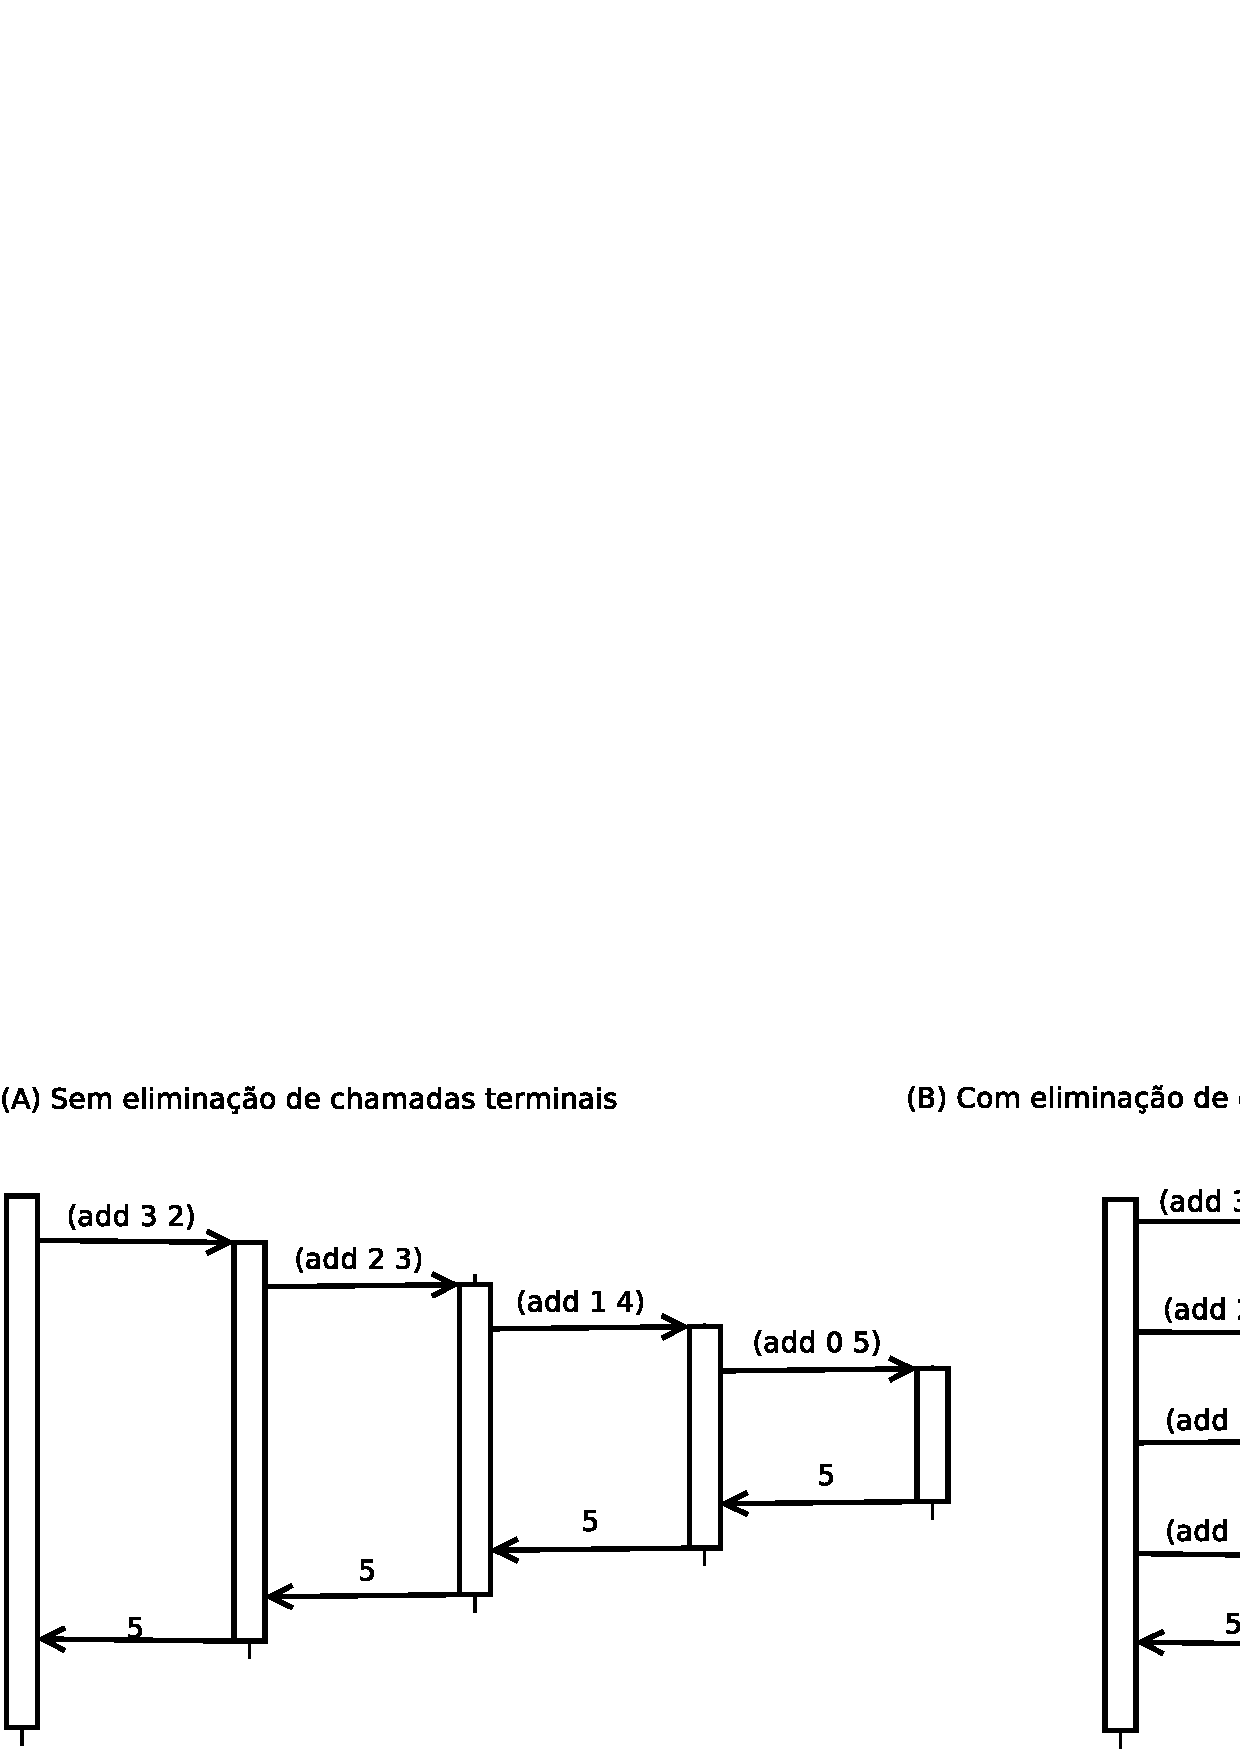
\includegraphics[width=0.9\textwidth]{../images/tail-call-elimination.pdf}
\caption{Tempo de vida de registros de ativação em relação a chamadas terminais}
\label{fig:tail-call-elimination}
\end{figure}

Quando uma implementação \textit{Scheme} se depara com uma aplicação de chamada
de função terminal, esta deve evitar criar um novo registro de ativação e
reutilizar o registro de ativação da função em vigor como o registro de
ativação da função prestes a ser chamada. Recursões em que a chamada recursiva
em si é considerada terminal, por meio da eliminação de chamadas terminais,
utilizam quantidade constante de memória na pilha de ativações de funções.

\subsection{Representação textual}

Como membro da família Lisp, código
\textit{Scheme} é representado textualmente por listas de elementos separados
por espaço em branco, agrupados por parênteses, que denotam um formato abstrato
conhecido como Expressões-S (abreviação de Expressões Simbólicas). Expressões-S
podem ser definidas recursivamente da seguinte forma:

\begin{itemize}

\item Um elemento atômico (número, símbolo ou outro literal da linguagem) é uma
Expressão-S;

\item Uma lista de Expressões-S é uma Expressão-S.

\end{itemize}

Ainda em conformidade com a família Lisp, \textit{Scheme} adota a notação
polonesa (ou notação de prefixos), na qual as listas representam operações em
que o primeiro elemento é o operador, que pode ser uma função ou uma forma
sintática, e os demais elementos são parâmetros para a operação.

\subsection{Funções e Formas Sintáticas}

Embora a sintaxe para aplicação de funções ou formas sintáticas seja idêntica,
é importante ressaltar as diferenças básicas entre os dois tipos de operações,
já que possuem semânticas bastante distintas. A distinção entre funções e
formas sintáticas pode ser traçada com base na fase da computação em que são
avaliados e na estratégia de avaliação de parâmetros, como visto na tabela
\ref{table:functions-vs-special-forms}.

É interessante notar que do ponto de vista de uma implementação \textit{Scheme}
formas sintáticas primitivas, como \sctt{if} ou \sctt{lambda}, possuem
tratamento semântico idêntico ao das formas sintáticas derivadas definidas pelo
usuário, exceto pelo fato que as primeiras são tratadas diretamente pelo
compilador e as segundas são gerenciadas pelo mecanismo de macros.

\begin{table}[h!]
 \begin{center}
  \begin{tabular} { | c | p{4cm} | p{4cm} | }
   \hline
                        & \textbf{Funções} & \textbf{Formas Sintáticas} \\ \hline
    \textbf{Avaliação de Parâmetros} & Todos os parâmetros são avaliados antes da chamada da função propriamente dita. & Nenhum dos parâmetros é avaliado, a forma sintática é executada com a representação em lista do código. \\ \hline
    \textbf{Fase da Avaliação} & São avaliadas durante a execução do programa. & São avaliadas antes do código ser executado, durante a compilação ou imediatamente antes da interpretação. \\ \hline
  \end{tabular}
 \end{center}
 \caption{Diferenças entre Funções e Formas Sintáticas} 
 \label{table:functions-vs-special-forms}
\end{table}

\subsection{Processamento de listas e macros}

Scheme herda dos Lisps anteriores um grande número de operações sobre listas, e
a utilização de Expressões-S (estruturas baseadas em listas) faz com que seja
fácil manipular representações em Expressão-S de código \textit{Scheme},
utilizando a própria linguagem. Esta propriedade, aliada à capacidade do
programador de definir código de funções ou substituições a serem aplicadas no
código anteriormente à compilação ou interpretação, leva a um poderoso sistema
de macros que permite ao programador criar novas formas sintáticas que são
convertidas para formas primitivas da linguagem. Desta maneira, o fato de ser
uma linguagem minimalista não interfere com a expressividade do programador
final, que em geral lida com expressões mais complexas abstraídas por trás de
formas sintáticas derivadas.

A criação de macros, embora uma das partes mais difíceis da linguagem em um
primeiro contato com \textit{Scheme}, se baseia em uma idéia simples: O
programador pode indicar ao compilador palavras-chave que serão identificadas
quando encontradas como primeiro elemento de uma forma aplicativa (expressão
entre parênteses) e associar transformações às mesmas. Estas transformações
deverão ser executadas pelo compilador quando uma forma aplicativa iniciando
por uma das palavras-chave definidas for encontrada, utilizando como entrada a
forma aplicativa encontrada no código fonte como parâmetro. Esta execução deve
retornam uma nova Expressão-S que o compilador substituirá pela forma
aplicativa inicial.  Desta forma, um programador pode informar ao compilador a
maneira (a transformação associada à palavra-chave) que deverá ser utilizada
para tratar formas sintáticas inicialmente desconhecidas, reduzindo-as para
formas sintáticas primitivas que o compilador conhece.

Historicamente, dois mecanismos principais de macros foram utilizados em
\textit{Scheme} e outras linguagens da família Lisp: macros procedurais e
macros baseadas em regras. \textit{Scheme} como definida pelo \acs{R7RS}
oferece suporte apenas a macros baseadas em regras.

As macros procedurais são aquelas em que o programador define a transformação a
ser aplicada em termos de código \textit{Scheme}, recebendo a forma sintática
original em seu formato de Expressão-S e manipulando-a como necessário para
atingir a forma final desejada. Já as macros baseadas em regras são descritas
em uma linguagem auxiliar de reconhecimento de padrões e suas regras de
substituição são utilizadas para transformar uma Expressão-S que case com uma
das regras pelo resultado definido para a regra indicada. 

\subsection{Escopo de variáveis}

\textit{Scheme} foge da tradição entre linguagens anteriores da família Lisp
por adotar um modelo de escopo léxico, ou estático, no qual o escopo de uma
variável pode sempre ser determinado pela simples análise do texto do programa.
Partindo do ponto em que a variável é referenciada, utilizando escopo léxico, e
voltando na estrutura do código é sempre possível encontrar o ponto em que esta
é declarada ou, caso não seja possível (ou seja, esta variável é uma variável
livre no contexto atual), esta tem de ser uma variável global -- ou um erro por
parte do programador, visto que então a variável não estaria declarada em lugar
algum.

Tradicionalmente, no entanto, dialetos Lisp implementavam uma estratégia de
escopo dinâmico em que uma variável livre estava vinculada à declaração da mais
recente variável de mesmo nome no contexto dinâmico da pilha de chamadas
anteriores. A diferença entre as estratégias de escopo léxico e dinâmico é 
exemplificado a seguir com base no código abaixo:

\begin{lstlisting}
    (define x 0)
    
    (define (func1 n) 
      (+ n x))
    
    (define (func2 n) 
      (let ((x 1))
        (func1 n)))
\end{lstlisting}

Caso se observe o código acima sob a ótica de uma implementação Lisp com
estratégia de escopo dinâmico, ao se executar a uma chamada à função
\sctt{func2} passando um número qualquer \sctt{n} como parâmetro, o resultado
encontrado seria o mesmo de executar a expressão \texttt{(+ n 1)}, visto que o
valor encontrado na variável \sctt{x} no corpo da função \sctt{func1} é
vinculado ao valor mais próximo de \sctt{x} encontrado na estrutura dinâmica de
registros de ativação das funções executadas, ou seja, o valor em \sctt{func2}.

No entanto, sob o ponto de vista de uma estratégia de escopo estático, o
resultado encontrado é equivalente a retornar o parâmetro diretamente, na
verdade a soma deste parâmetro ao valor 0, visto que o vínculo dado a \sctt{x}
em \sctt{func1} é sempre o encontrado no escopo durante a análise estática do
código sem informações de tempo de execução, ou seja, a variável global
definida na linha 1.

De acordo com Sussman e Steele[1], esta mudança fez com que o tratamento de
variáveis livres em um a expressão fosse semanticamente análogo ao dado no
formalismo do Cálculo Lambda, fornecendo um bom modelo computacional para
experimentação com o Cálculo Lambda. Novamente de acordo com os criadores da
linguagem [1], esta proximidade com o Cálculo Lambda foi um dos motivos
principais para a utilização futura de \textit{Scheme} como uma linguagem de
ensino e experimentação de conceitos de linguagens de programação.

\subsection{Closures}

A mudança para o escopo léxico, associada à possibilidade de criação e
manipulação de funções como objetos em tempo de execução, faz com que seja
possível gerar \textit{closures}, ou seja: funções que capturam o vínculo de
variáveis como estavam no momento em que a função foi declarada em tempo de
execução e carregam estes vínculos consigo, podendo manipulá-los e modificá-los
como quiser. Esta técnica é largamente utilizada em \textit{Scheme} para criar
unidades de código que contém tanto código de função como estado de variáveis,
de forma análoga a alguns tipos de objetos de uma linguagem orientada a
objetos.

Um exemplo simples de closure, para demonstrar o conceito, é dado no código a
seguir, em que uma função (\sctt{multiplicador}) recebe como parâmetro um
número \sctt{n} e retorna uma função de um parâmetro \sctt{x} que multiplica
todo \sctt{x} passado pelo \sctt{n} recebido por \sctt{multiplicador}. Pode-se
dizer que a função criada pela \textit{expressão lambda} contida em
\sctt{multiplicador} cria uma closure sobre o vínculo associado ao nome \sctt{n}
no escopo em que foi avaliada, e este vínculo é acessado sempre que a função
resultante desta \textit{expressão lambda} for aplicada.

\begin{lstlisting}
    (define (multiplicador n)
       (lambda (x) (* n x)))
\end{lstlisting}

Como exemplo, pode-se observar o resultado de uma interação com o interpretador
na figura \ref{fig:interacao-closure}.

\begin{figure}[h!]
\begin{lstlisting}[numbers=none]
    Welcome to Stutter.
    
    > (define (multiplicador n) 
        (lambda (x) (* n x)))
    #U
    
    > multiplicador
    User defined function at 0x0x7f9b3aa75a18
    
    > (define t5 (multiplicador 5))
    #U
    
    > (define t10 (multiplicador 10))
    #U
    
    > (t5 3)
    15
    
    > (t10 3)
    30
\end{lstlisting}
\caption{Interação com o Interpretador exemplificando efeitos de closures.}
\label{fig:interacao-closure}
\end{figure}

\subsection{Continuações como objetos de primeira classe}
\label{ss:continuacoes}

Uma continuação de uma computação qualquer pode ser vista como um par composto
pelo contexto em que aquela computação está acontecendo e o lugar para o qual
esta computação deve retornar o seu valor após ser avaliada. Por exemplo, no
trecho de código seguir:

\begin{lstlisting}
(set! x (+ 3 2))

\end{lstlisting}

Pode-se dizer que a continuação da expressão ``\texttt{2}'' é composta pelo
contexto dos vínculos de variáveis presentes durante sua execução (que contém,
entre outras coisas os valores das variáveis ``\texttt{x}'' e ``\texttt{+}''),
a cadeia de registros de ativação de funções que leva ao momento em que esta
expressão está sendo executada e uma referência ao ponto da computação para o
qual o valor deve ser entregue (neste caso a expressão ``\texttt{(+ 3 \_)}'',
onde ``\texttt{\_}'' representa onde este valor vai ser entregue). De forma
mais simples, uma continuação é uma \textit{procedure} que representa a idéia
dos ``passos seguintes'' de uma computação.

\textit{Scheme} foi a primeira linguagem de programação a tratar continuações
como objetos de primeira classe, ou seja: um progamador pode obter a
continuação atual, passar continuações como parâmetros, armazená-las em
variáveis, retornar como valor de uma função e invocá-las para retornar ao
ponto da computação que elas descrevem. Isto é feito por meio da primitiva
\texttt{call-with-current-continuation}, normalmente abreviada
\texttt{call/cc}.  Esta primitiva recebe uma função de apenas um parâmetro e
invoca esta função passando a continuação da computação no momento em que foi
chamada; e retorna o valor retornado pela função que recebeu, na primeira
chamada, ou os valores passados para a continuação sempre que esta for
invocada. O exemplo a seguir utiliza a obtenção da continuação atual para
simular o efeito da operação``\texttt{return}'' em outras linguagens:

\begin{lstlisting}
    (define (find-return n lst accept?)
       (call/cc 
         (lambda (return)
            (for-each (lambda (element)
                        (if (accept? element)
                           (return element)))
                      lst)
            #F)))
\end{lstlisting}

A função acima, \texttt{find-return}, itera por uma lista procurando pelo 
primeiro elemento que satisfaça ao predicado \texttt{accept?}. Embora seja uma 
forma estranha de programar \texttt{Scheme}, demonstra como o conceito de 
continuações como objetos de primeira classe pode ser utilizado para simular
a instrução ``\texttt{return}'' como aparece em outras linguagens: a continuação
da chamada a \texttt{call/cc} é salva como a variável \texttt{return} e é 
invocada quando o elemento é encontrado. 

Formas mais complexas de utilização de continuações, aliadas ao fato de que o
\textit{boilerplate} pode ser escondido por trás de macros mais convenientes,
tornam as continuações uma fonte de estruturas de controle das mais diversas.
Por exemplo, o mecanismo de tratamento de exceções utilizado em \texttt{Scheme}
pode ser totalmente implementado em termos de continuações de primeira classe.

\subsection{Quote}
\label{ss:quote}

Como em \textit{Scheme} a mesma sintaxe é utilizada para representar uma lista
de dados como para representar uma aplicação de função ou forma sintática,
assim como a mesma sintaxe é utilizada para repersentar símbolos como objetos e
símbolos como referência a variáveis, é necessário ter um mecanismo pelo qual
descrever elementos a serem usados como dado em um programa que não devem
sofrer nenhuma avaliação pelo ambiente. A expressão \texttt{quote} supre essa
necessidade.

Na maior parte dos casos, uma referência a uma lista no código, como
\texttt{(foo 10)} significa uma aplicação de função a seus parâmetros. Em 
algumas situações no entanto, pode ser interessante, por exemplo, indicar a lista
composta pelo símbolo \texttt{foo} e o número inteiro \texttt{10}, nestes
casos pode-se utilizar a expressão \texttt{(quote (foo 10))} que pode ser 
abreviada simplesmente como \texttt{'(print 10)}. 

O mesmo vale para quaisquer outros valores \textit{Scheme}. Os que possuem
algum significado específico, diferente do próprio valor, na sintaxe da
linguagem quando \textit{citados} (em tradução livre do termo original
\textit{quoted}) serão ignorados pelo compilador, sendo utilizados como
constantes. Os valores que não possuem significado especial algum além do
próprio valor são considerados automaticamente \textit{citados}, de forma que
aplicar a operação \texttt{quote} nestes não faz diferença alguma.

\subsection{Quasiquote}
\label{ss:quasiquote}

Parecido com o mecanismo disponível pela expressão \texttt{quote}, a expressão
\texttt{quasiquote} permite criar dados com a sintaxe de lista, utilizando
durante sua definição as expressões \texttt{unquote} e \texttt{unquote-splicing}
para misturar dados que devem ser utilizados como constantes não interpretadas
na lista final com dados que devem ser interpretador antes de ter seu valor 
utilizado na criação da lista final. As expressões \texttt{unquote} e 
\texttt{unquote-splicing} funcionam da seguinte maneira:

\begin{itemize}

\item \texttt{unquote} coloca o valor da próxima Expressão-S, interpretada como
seria caso não houvesse quote, como um elemento da Expressão-S sendo gerada.
Por exemplo, \texttt{(quasiquote 1 2 (unquote (list 3 4)))} é equivalente à lista
\texttt{'(1 2 (3 4))}.

\item \texttt{unquote-splicing} coloca o valor da próxima Expressão-S, em geral
uma lista, de forma que todos os seus elementos estejam presentes diretamente
na Expressão-S que a engloba. Por exemplo, \texttt{(quasiquote 1 2
(unquote-splicing (list 3 4)))} é equivalente à lista \texttt{(1 2 3 4)}.

\end{itemize}

As expressões \texttt{quasiquote}, \texttt{unquote} e \texttt{unquote-splicing}
podem ser abreviadas respectivamente pelos caracteres \textit{backtick}
(\texttt{`}), vírgula (\texttt{,}) e a combinação vírgula-arroba (\texttt{,@}).





\chapter{Estratégia de Implementação}
\label{cap:estrategia}

\vfill{}
\begin{flushright}{}
``\emph{The world is moving so fast these days that the man who says it
can't be done is generally interrupted by someone doing it.}''\\
{\small Elbert Green Hubbard}
\end{flushright}{\small \par}
\vfill{}

Neste capítulo são apresentados a motivação e os objetivos deste projeto, uma
lista de trabalhos relacionados e a estrutura da monografia.
\newpage


\section{Visão Geral}
\label{sec:estrategia_geral}

Para a implementação do interpretador, as tarefas necessárias para a
interpretagção, do código fonte ao resultado final de uma computação, foram
divididas entre quatro módulos: o Leitor, o Compilador, a Máquina Virtual e o
Sistema de Gerência de Memória.


O Leitor é responsável pela primeira etapa antes da compilação propriamente
dita: traduzir o código em formato textual fornecido pelo usuário para
Expressões-S. Durante a fase de leitura é realizada a análise léxica, bem como
a formação das listas que compõe a estrutura de um programa Scheme, que
corresponde a parte da análise sintática. O módulo Leitor é descrito em mais
detalhes na seção \ref{sec:leitor}.

Utilizando as Expressões-S geradas pelo Leitor, identifica qual estrutura da
linguagem cada Expressão-S representa, reconhece instâncias de macros que devem
ser traduzidas para as definições dadas pelo usuário e finalmente gera o código
que deve ser executado para avaliação das expressões fornecidas. Como a
tradução de macros acontece antes da geração de código, esta fase fica
significativamente mais simples, precisando apenas lidar com as poucas
estruturas primitivas que a linguagem define, deixando as demais para serem
reduzidas às estruturas primitivas por meio de macros. Na seção
\ref{sec:compilador} são fornecidos mais detalhes sobre o Compilador, bem como
seus sub-módulos: o Leitor e o Sistema de Macros.

A Máquina Virtual, então, é encarregada de avaliar as operações codificadas em
instruções básicas, utilizando o código gerado pelo compilador, e retornar o
valor desta avaliação. Para tanto, esta depende de um contexto de execução,
composto das ligações presentes no escopo global. Informações extras de
contexto, como os escopos locais e estado da pilha de controle, entre outras,
são mantidas e serão discutidas, junto com uma descrição detalhada da Máquina
Virtual, na seção \ref{sec:maquina-virtual}.

Uma representação simplificada do funcionamento do interpretador, baseada na descrição acima, pode
ser vista na figura \ref{fig:visao-geral-implementacao}.

\begin{figure}[h!]
\centering
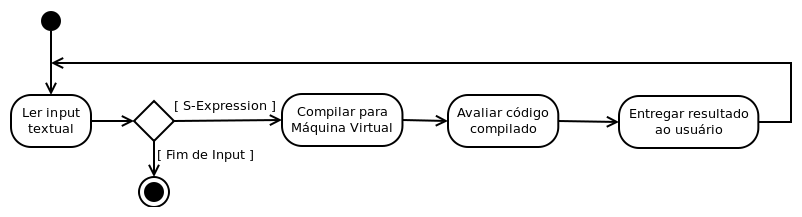
\includegraphics[width=0.9\textwidth]{../images/visao-geral-implementacao.pdf}
\caption{Visão geral do funcionamento interno do interpretador}
\label{fig:visao-geral-implementacao}
\end{figure}

Os módulos descritos acima são implementados sobre o sistema de Gerência de
Memória. A Gerência de Memória é baseada em uma implementação simples do
algoritmo de Mark \& Sweep [17], em que a memória livre é armazenada como uma
lista encadeada de nós de memória de tamanho único (neste caso, 24 bytes). Com
a ajuda de um conhecimento mais íntimo da máquina virtual em questão, o sistema
de gerência de memória pode então, quando necessário, identificar quais nós de
memória estão em uso e liberar para uso posterior todos os demais. Na seção
\ref{sec:memoria} detalharemos o sistema de memória, embora uma compreensão
completa do mesmo só seja possível após indicarmos quais partes da máquina
virtual estão envolvidas no processo de identificar quais nós de memória estão
em uso.

Podemos ter então, quebrando o trabalho do compilador em seus sub módulos
separadamente, uma visão geral da arquitetura do Interpretador, em como os
módulos se relacionam na figura \ref{fig:camadas} e de como se dá, em detalhes, o
processo de interpretação de uma expressão Scheme dada como entrada ao
interpretador na figura \ref{fig:atividades}

\begin{figure}[h!]
\centering
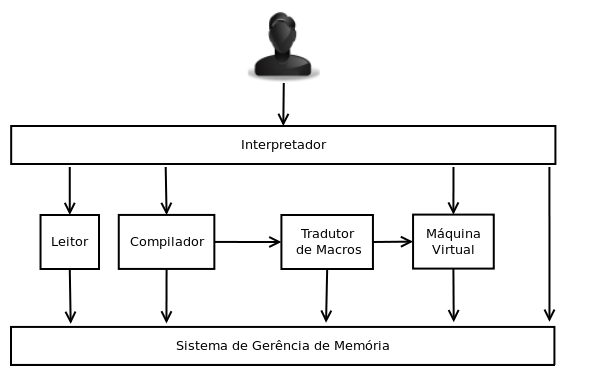
\includegraphics[width=0.9\textwidth]{../images/camadas.pdf}
\caption{Estrutura e relacionamento entre os módulos do interpretador}
\label{fig:camadas}
\end{figure}

\begin{figure}[h!]
\centering
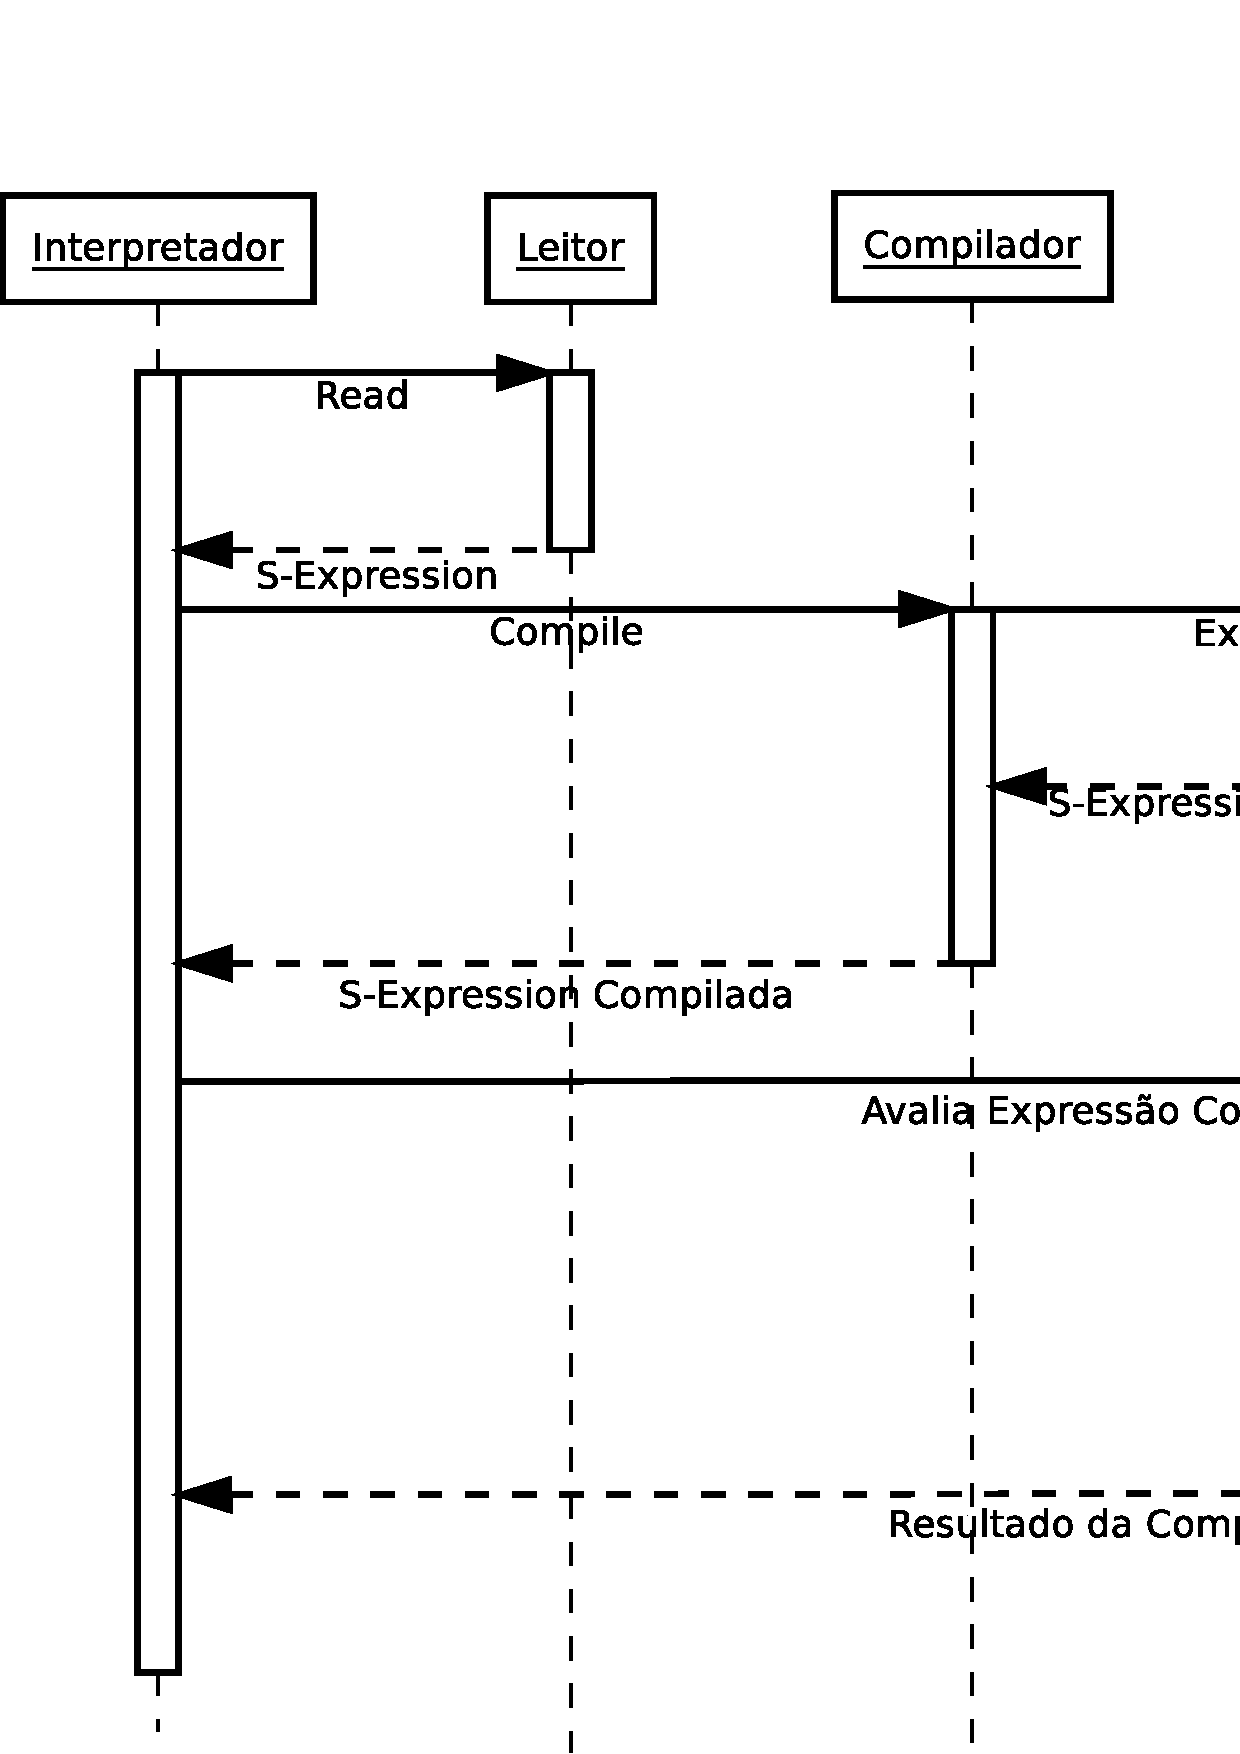
\includegraphics[width=0.9\textwidth]{../images/atividades.pdf}
\caption{Processo interno de interpretação}
\label{fig:atividades}
\end{figure}

A implementação do interpretador baseado no esquema descrito acima se dá em um
ambiente de duas linguagens: C++ e Scheme.

A estrutura básica do interpretador, até o ponto em que este é capaz de
interpretar um pequeno conjunto de operações básicas, é feito em C++. Esta
estrutura inclui todo o mecanismo de gerência de memória, o leitor, o
compilador para as estruturas sintáticas primitivas e a máquina virtual, além
de um pequeno conjunto de funções primitivas que são mais fácilmente
implementadas em C++ por apenas delegarem o trabalho para funções e operadores
primmitivos desta linguagem.

A partir deste ponto, as demais estruturas sintáticas são escritas na forma de
macros em Scheme e diversas funções da biblioteca são implementadas em código
Scheme que roda no próprio interpretador. 

Utilizando uma análise de número de linhas de código, que não é exatamente
representativa dada a diferença de expressividade das duas linguagens,
aproximadamente 88\% da implementação é feita em C++, enquanto que os 12\%
restantes são feitos em Scheme.




\section{Sistema de Gerência de Memória}
\label{sec:memoria}

Embora não seja exatamente um requerimento da R7RSsmall, esta implementação
possui também um mecanismo de gerência de memória automatizado, o que definiu
em diversas formas as escolhas utilizadas para representação dos valores em
tempo de execução nesta implementação. Além disso, historicamente Lisp está tão
intimamente ligada à gerência automatica de memória, visto que foi a primeira
linguagem de programação a utilizar a técnica[20], que a escolha por incluir um
mecanismo de gerência automática de memória se deu pelo interesse em descrever
o mesmo algoritmo utilizado por McCarthy em sua implementação original.

Em especial, existem dois tipos de valores, divididos por necessitarem ou não
de alocação de memória dinâmica. Entre os valores que não necessitam de
alocação de memória dinâmica, chamados daqui em diante de valores imediatos,
encontram-se os inteiros, booleanos, caracteres e alguns valores especiais como
o marcador de lista vazia. Estes, são implementados na forma de "ponteiros
etiquetados" (tagged pointers), em que os dados ocupam os 62 bits mais
significativos de uma palavra de 64 bits, e os 2 bits menos significativos são
utilizados para identificar os valores como imediatos, identificação preliminar
do tipo e diferenciar estes valores dos demais ponteiros no sistema.

Os demais, como funções, strings, pares e quaisquer estruturas de dados
complexas, são implementados seguindo uma estrutura de dados comum a todos, de
forma a simplificar a implementação do mecanismo de gerência de memória.
Nestes, os 2 bits menos significativos têm obrigatóriamente o valor zero,
criando a necessidade de um alinhamento de 4 bytes para cada objeto alocado em
memória. A estrutura utilizada para estes valores complexos é a descrita a
seguir e pode ser vista na figura \ref{fig:celula}:

Uma palavra de 64 bits é utilizada para manter informações de tipo, dados
relacionados à gerência de memória e se o objeto armazenado pode ser
modificado. Entre estes, deve-se ressaltar os dados de gerência de memória que
indicam:

\begin{itemize}

\item se o objeto foi visitado pelo sistema de gerência de memória durante a
coleta (\sctt{gc\_has\_mark});

\item  se o objeto está em uso pelo sistema (\sctt{gc\_is\_in\_use});

\item  se o mecanismo de gerência de memória deve analisar seu filho esquerdo
(\sctt{mark\_policy\_first}) e/ou seu filho direito
(\sctt{mark\_policy\_second});

\item  ou se a memória para este objeto nunca deve ser liberada
(\sctt{gc\_always\_marked}).

\end{itemize}

Além destas informações, um conjunto de bits é utilizado para manter a
informação sobre o tipo destes objetos, para questões de despacho de funções e
checagem de tipos. Oito bits foram utilizados para este fim, embora devido ao
grande espaço não utilizado na estrutura mais possam ser utilizados para
estender o mecanismo de tipos caso seja necessário.

Em seguida, duas outras palavras de 64 bits são utilizadas para armazenar as
demais partes da estrutura de dados. Estas duas palavras (chamados daqui em diante
simplesmente de  \textit{slots}) armazenam valores arbitrários do sistema, usando a mesma técnica
de tagged pointers mencionada anteriormente, em que valores imediatos são
armazenados diretamente e valores complexos são armazenados como ponteiros para
outras estruturas idênticas às aqui descritas. 

Esta estrutura simples representa diretamente a estrutura de dados mais
utilizada em um dialeto Lisp: a "célula cons" que é utilizada para, entre
outras coisas, representar listas, como a representação interna do código
fonte. Uma célula cons nada mais é que um par de dois outros valores quaisquer
da linguagem. Esta estrutura é utilizada para todos os demais valores que não
podem ser representados como valores imediatos, o que é bom o suficiente já que
o objetivo desta implementação não é o de otimizar para espaço ou tempo.

\begin{figure}[h!]
\centering
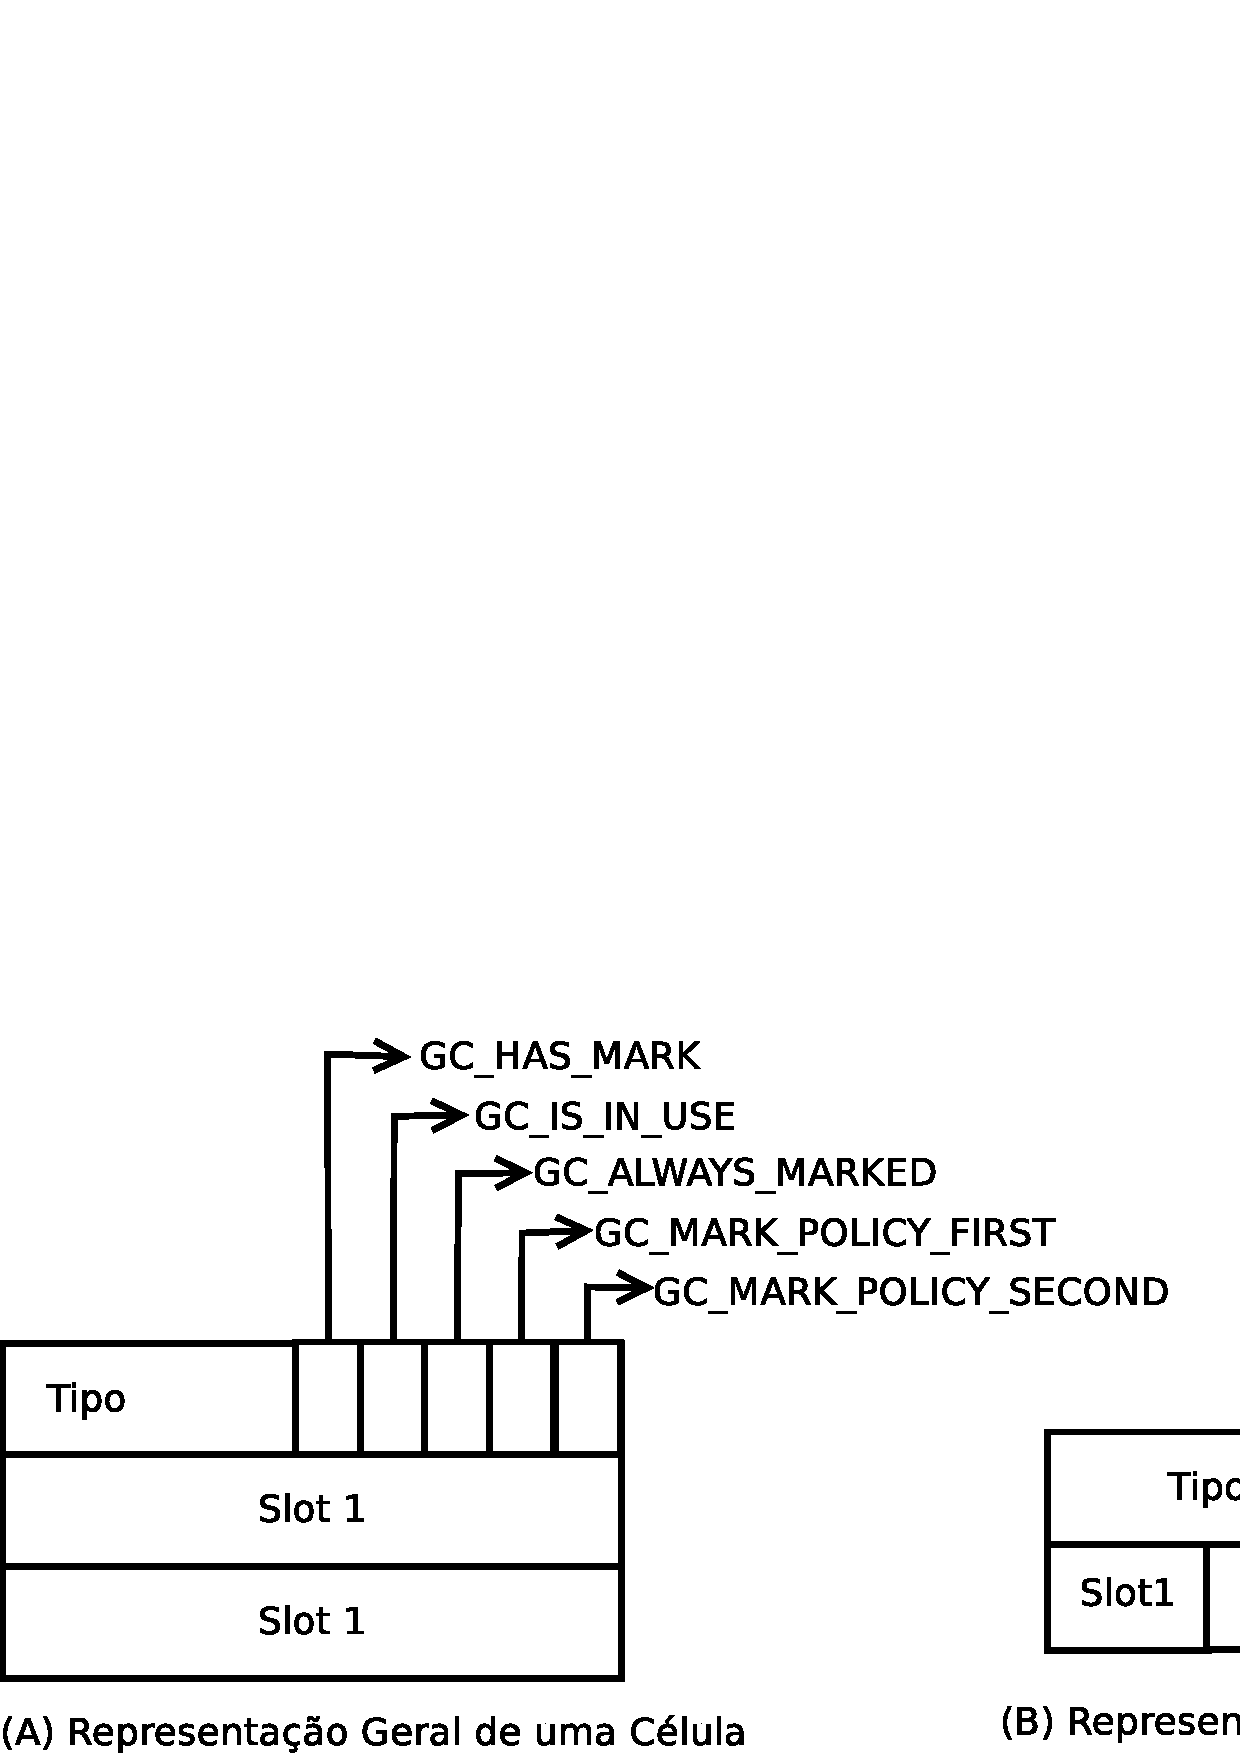
\includegraphics[width=0.9\textwidth]{../images/celula.pdf}
\caption{Duas visões para a estrutura de célula de memória utilizada}
\label{fig:celula}
\end{figure}


Como todos os valores não imediatos são representados utilizando esta
estrutura de armazenamento duplo em \textit{slots}, em alguns casos apenas um dos \textit{slots}
de armazenamento é utilizado, em outros casos ambos. Na figura \ref{fig:memoria}
pode-se verificar alguns exemplos de como a memória é estruturada quando
representa alguns objetos.


\begin{figure}[h!]
\centering
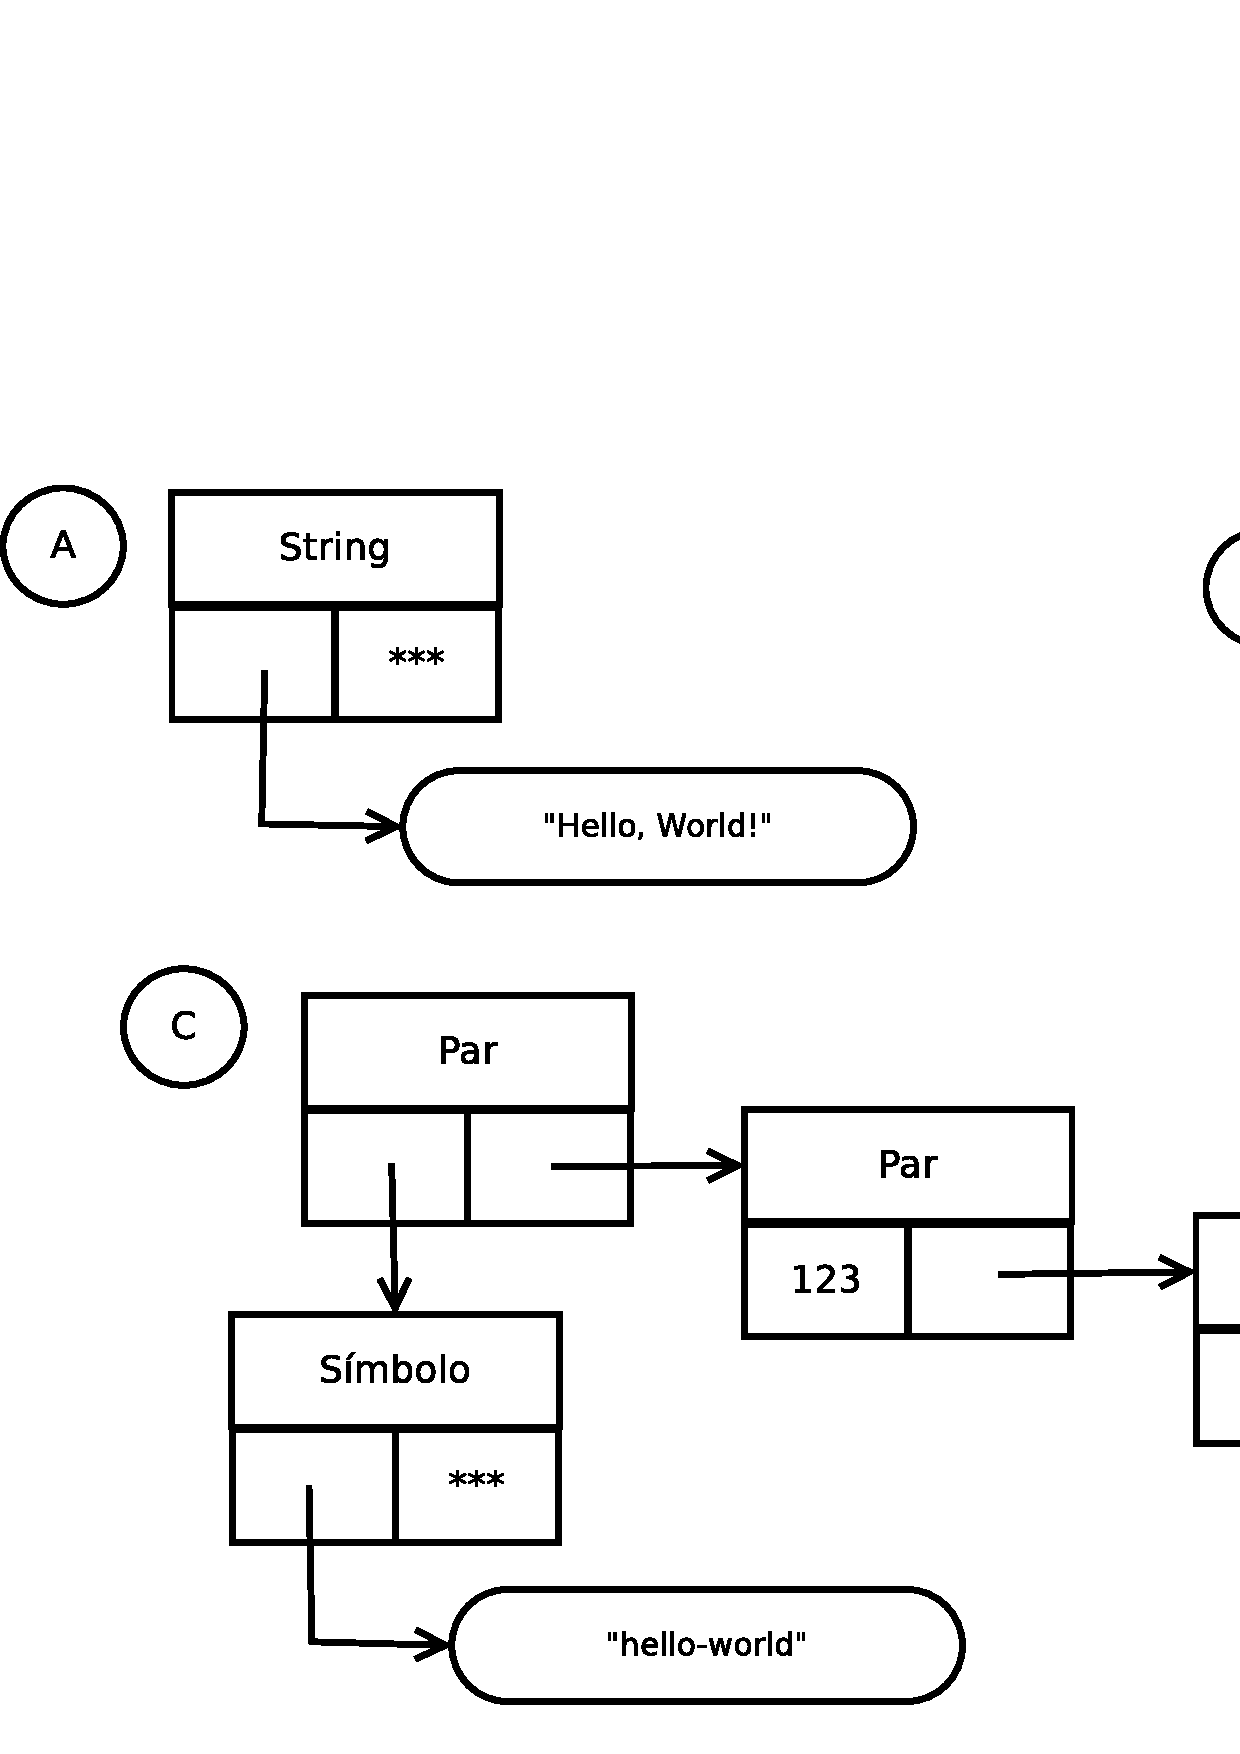
\includegraphics[width=1\textwidth]{../images/memoria.pdf}
\caption{Estrutura de objetos em memória. (A) uma string; (B) uma função
         primitiva; (C) uma lista com um símbolo e alguns valores imediatos.}
\label{fig:memoria}
\end{figure}

Dado que todos os valores armazenados por meio de alocações dinâmicas possuem o
mesmo formato e é trivialmente possível identificar ponteiros para outros
objetos na estrutura utilizada, fica simples implementar um mecanismo de
gerência de memória. O algoritmo utilizado é o mesmo descrito por John McCarthy
em sua implementação original de Lisp[20], e consiste dos seguintes passos:

\begin{itemize}

\item Inicialize a memória como um bloco de elementos "livres", prontos a serem
utilizados;
 
\item Configure este bloco de forma que o segundo \textit{slot} de cada elemento aponte
para o próximo, formando uma lista encadeada de elementos livres;
 
\item A cada nova alocação necessária, obtenha um elemento da lista de
elementos livres;
 
\item Quando não houver mais elementos livres, identifique os elementos que
estão em uso e marque-os (fase de marcação);
 
\item Após marcar os elementos em uso, varra a área de memória utilizada
retornando todos os elementos que não estão sendo utilizados para a lista de
elementos livres (fase de varredura).

\end{itemize}

Para identificar os elementos que estão em uso, basta seguir as cadeias de
referências dos \textit{slots} da estrutura descrita acima, a partir dos registradores
da máquina virtual e de algumas outras estruturas auxiliares, marcando todos os
elementos encontrados como sendo utilizados.

Dado que os elementos são alocados dentro de um ou mais blocos conhecidos de
memória, é fácil iterar por todos os elementos alocados, reinserindo-os na
lista de elementos livres se não estiverem marcados e desmarcando os que
estiverem, para deixar o estado geral da memória pronto para outro ciclo de
coleta.

Por questões de otimização uma flag (\sctt{gc\_always\_marked}) indica objetos
que não são varridos por gerenciarem a própria memória e nunca serem
desalocados após serem criados. E por haver valores que não ocupam ambos os
\textit{slots}, ou ainda por haver valores que guardam dados que não são controlados
pela gerência de memória nestes \textit{slots}, algumas flags
(\sctt{mark\_policy\_first}, \sctt{mark\_policy\_second}) controlam se é
necessário continuar o percurso por cada um dos \textit{slots} de um elemento.

Este modelo simples de gerência de memória, conhecido como Mark \& Sweep pelas
duas fases utilizadas[17], é suficiente para garantir que a máquina virtual
utilize plenamente a memória disponível antes de terminar por falta de
memória.


\section{Leitor}
\label{sec:leitor}

O módulo Leitor, uma parte tradicional da implementação de linguagens da família Lisp é responsável por receber um fluxo de texto e processá-lo para obter um fluxo de Expressões-S.

Sua primeira responsábilidade é a análise léxica da entrada, identificando os tokens no texto e transformando-os em representações de objetos atômicos no contexto das Expressões-S: constantes simbólicas, constantes numéricas e outras constantes além de pontuação como parênteses e ponto, e eliminar os comentários. 

Além da análise léxica, o Leitor vai um passo além, construindo as estruturas (listas) que compõem uma Expressão-S, agrupando os objetos de forma que todo o resto do processo de compilação não precise se preocupar com como a informação é armazenada textualmente, lidando apenas com Expressões-S.

Sua implementação é bastante simples: Utilizando o gerador de analisadores léxicos GNU Flex[18] é criada uma função inicial capaz de traduzir a entrada textual nos respectivos objetos atômicos e pontuação reconhecidos pela estrutura das Expressões-S. Neste ponto, a análise léxica é concluída. 

Uma segunda função, que é exposta para os demais módulos, é responsável por coordenar as chamadas à função gerada pelo GNU Flex e criar as estruturas recursivas de uma Expressão-S, as listas e sublistas.

Todas as estruturas criadas são alocadas com a ajuda do Sistema de Gerência de Memória, e entre uma alocação e outra, são protegidas usando a pilha de proteção de memória, para evitar que uma chamada à coleta de lixo durante a execução de uma chamada ao Leitor descarte memória que foi recentemente alocada mas ainda não está em uso pelo programa do ponto de vista da Máquina Virtual.





\section{Compilador}
\label{sec:compilador}

A estratégia utilizada para o compilador é derivada de um compilador utilizado como exemplo por Kent Dybvig em sua tese de doutorado[19]. Este compilador, embora simples, sofre de algumas deficiências que serão discutidas adiante.

Durante a etapa de compilação traduzimos uma Expressão-S representando código Scheme para uma Expressão-S representando a implementação deste código nas instruções utilizadas pela máquina virtual. Observe que, como a compilação se dá em termos de Expressões-S como entrada, nada impede que um usuário forneça ao compilador uma Expressão-S que não é diretamente derivada da representação textual do programa. Esta informação será utilizada quando discutirmos o mecanismo de tradução de Macros.

Neste momento vamos abstrair o funcionamento do mecanismo de macros, dizendo apenas que antes de a compilação propriamente dita ter início, o Compilador invoca o sistema de macros para processar a Expressão-S recebida como entrada de forma a transformá-la em uma Expressão-S representando uma das poucas operações primitivas das quais o compilador tem conhecimento. Este fato simplifica muito a etapa de compilação, permitindo ao compilador se preocupar apenas com um número reduzido das estruturas sintáticas definidas no R7RS-small.

A estratégia de implementação utilizada é a mais ingênua possível. Com efeito, esta implementação não mantém informações de análise estática relacionadas a escopo, o que a faz incapaz de representar o mecanismo de macros definido pela linguagem Scheme. A implementação de um mecanismo alternativo de macros procedurais, compatível com os mecanismos tradicionais de outras linguagens da família Lisp, além de uma descrição das mudanças necessárias para se implementar o mecanismo de macros descrito por Scheme, são discutidos posteriormente na seção \ref{sec:macros}.

Dez tipos de expressão são reconhecidos pelo compilador: Referência a variável, constantes,  expressões literais, criação de procedimentos, condicionais, atribuições, definições, definições de macro, obtenção de continuação e aplicação de função. A partir destes tipos primitivos de expressão, com a ajuda do mecanismo de macros, todas as outras estruturas sintáticas da linguagem são construídas, simplificando significativamente o projeto do compilador.

O processo de compilação inicia-se com dois parâmetros: a expressão a ser compilada e a próxima etapa da computação que está sendo efetuada. Quando estamos realizando a compilação de uma expressão no escopo mais alto, esta próxima etapa normalmente é um pedaço de código pré compilado correspondendo à instrução Halt da máquina virtual. Esta expressão representando a próxima etapa da computação pode então ser utilizada para compor o parâmetro das instruções da máquina virtual que indica qual a próxima instrução a ser executada.

% TODO [7]: Terminar esta seção.




\section{Máquina Virtual}
\label{sec:maquina-virtual}

A máquina virtual utilizada é baseada na arquitetura de máquina virtual
\sctt{secd} descrita por Peter Landin [Landin 1964] com pequenas alterações nos
registradores e instruções propostas por Kent Dybvig em sua tese de
doutorado[19]. Esta, como a de Landin, utiliza uma estrutura baseada em pilha,
com um pequeno número de registradores que apontam para memória organizada em
listas encadeadas. 

A estrutura da máquina é bastante simples: cinco registradores e 14 instruções.
Os registradores são todos baseados em memória organizada como listas, enquanto
que as instruções, em sua maioria, compartilham uma peculiaridade: Recebem como parâmetro
o código que deverá ser executado ao fim da instrução em questão. Algumas
exceções óbvias são as instruções \sctt{halt}, que termina a operação da
máquina e obviamente não recebe código algum para continuar, e \sctt{test}, que
decide entre duas linhas diferentes e portanto recebe dois parâmetros de código
para escolher executar ao fim da mesma.

Esta propriedade de representar o fluxo de controle de instruções
explícitamente na forma de parâmetros para todas as instruções simplifica
significativamente a implementação de duas das mais complexas funcionalidades
da linguagem: A obrigatoriedade de eliminar as chamadas terminais e a criação e
aplicação de continuações em tempo de execução.

Levando-se em consideração a simplicidade do código necessário para se
implementar a máquina virtual \sctt{secd} (aproximadamente 350 linhas de código
em C++) e o fato de ela tornar trivial a implementação das duas funcionalidades
mais complexas, esta foi escolhida para a implementação da fase de
interpretação propriamente dita neste interpretador. Nas sessões
\ref{ss:registradores} e \ref{ss:instrucoes} são detalhados os registradores e
instruções que compõem esta máquina.

\subsection{Registradores}
\label{ss:registradores}

O estado interno da máquina é composto pelos seus cinco registradores: os
quatro originais descritos por Landin, que dão o nome à máquina (\sctt{stack},
\sctt{environment}, \sctt{code} e \sctt{dump}), acrescidos de um
\sctt{acumulador}.

\begin{itemize}

\item O registrador \sctt{stack}, que aponta para uma lista encadeada que
armazena temporariamente os valores intermediários que serão ser passados para
chamadas de funções como parâmetros. 

\item Na arquitetura original não havia a presença de um \sctt{acumulador}, que
foi utilizado apenas para simplificar a codificação de algumas etapas, e
poderia perfeitamente ser substituído pelo uso judicioso do topo da pilha para
esta função. Este serve apenas para guardar resultados intermediários de forma
separada da pilha de parâmetros guardada na \sctt{stack}. 

\item O registrador \sctt{environment} aponta para uma lista composta dos
níveis de vínculos de variáveis válidos no escopo atual, estendendo-se até que
o escopo global é atingido por último. São armazenados de forma encadeada, com
cada contexto possuindo um ponteiro para o contexto no qual foi criado.

\item O registrador \sctt{code} aponta para uma representação da próxima
instrução a ser executada e pode ser visto como um análogo ao contador de
programa em uma arquitetura convencional de hardware, com a diferença que, no
modelo utilizado neste trabalho, cada instrução carrega consigo uma referência
explícita para a próxima instrução a ser executada, ao invés de depender de um
incremento implícito de contador.

\item O registrador \sctt{dump} mantém uma área de armazenamento temporário
para os outros registradores, exceto o \sctt{acumulador}, composto de um
conjunto \{\sctt{s}, \sctt{e}, \sctt{c}, \sctt{d}\} que, tendo como elemento o
conteúdo anterior do registrador \sctt{dump}, mantém uma pilha de contextos. É
internamente utilizado para manter a pilha de registros de ativação de chamadas
de função. 

\end{itemize}


\subsection{Representação visual dos Registradores}
\label{ss:registradores-visual}

Para atuar sobre o estado interno da máquina, são utilizadas 14 instruções que são
descritas a seguir. Na verdade, apenas 13 instruções seriam necessárias para
implementar a arquitetura proposta neste trabalho mas, devido a um problema de
projeto na fase do compilador uma instrução extra foi incluída de forma que a
máquina virtual possui algum conhecimento sobre o sistema de macros.

Durante a discussão das instruções a seguir, serão utilizadas as seguintes
representações para o conteúdo de cada registrador nos exemplos:

\begin{itemize}

\item Os registradores \sctt{stack} e \sctt{acumulador} serão representados
pela representação dos seus valores em Scheme, como descrito no apêndice 
\ref{apendice:sintaxe-leitor} com as seguintes adições:
 \begin{itemize}
 
 \item Closures serão representadas com o formato \texttt{closure(contexto;
parametros; corpo)}, em que \texttt{contexto} é representado como descrito
abaixo para o registrador \sctt{environment}, \texttt{parametros} é
representado como uma lista de átomos \textit{Scheme} e \texttt{corpo} é
representado como o descrito abaixo para o registrador \sctt{code}.

 \end{itemize}
\item Os contextos em \sctt{environment} serão representados por uma lista de
elementos delimitados por colchetes, em que o elemento mais à esquerda
representa o contexto mais recente. Elementos mais à direita indicam os demais
níveis de contextos no escopo atual, ou seja: \texttt{[a = 1, b = 2][c = 3][]}
representa o contexto em que as variáveis \texttt{a} e \texttt{b} têm valores
1, e 2, que é encadeado ao contexto em que \texttt{c} possui o valor 3. O
contexto vazio, \texttt{[]}, indica o escopo global com todos os vínculos
existentes neste.

\item O registrador \sctt{code} é representado pela notação de função
\textit{Scheme} com a exceção que parâmetros representados como palavras em
\sctt{maiúsculas} representam trechos de código da máquina virtual omitidos por
clareza.

\item O conteúdo de \sctt{dump} será representado usando a notação de cada um
dos registradores cujos valores armazena, delimitados por um par de chaves, com
registradores irrelevantes para o exemplo substituído por reticências. O
conteúdo de \sctt{dump} sem elementos será representado apenas como a lista
vazia \sctt{()}.

\end{itemize} 

Na figura \ref{fig:maquina} pode-se ver um exemplo da representação utilizada
para a máquina virtual como um todo durante a descrição das instruções a
seguir.

\begin{figure}[h!]
\centering
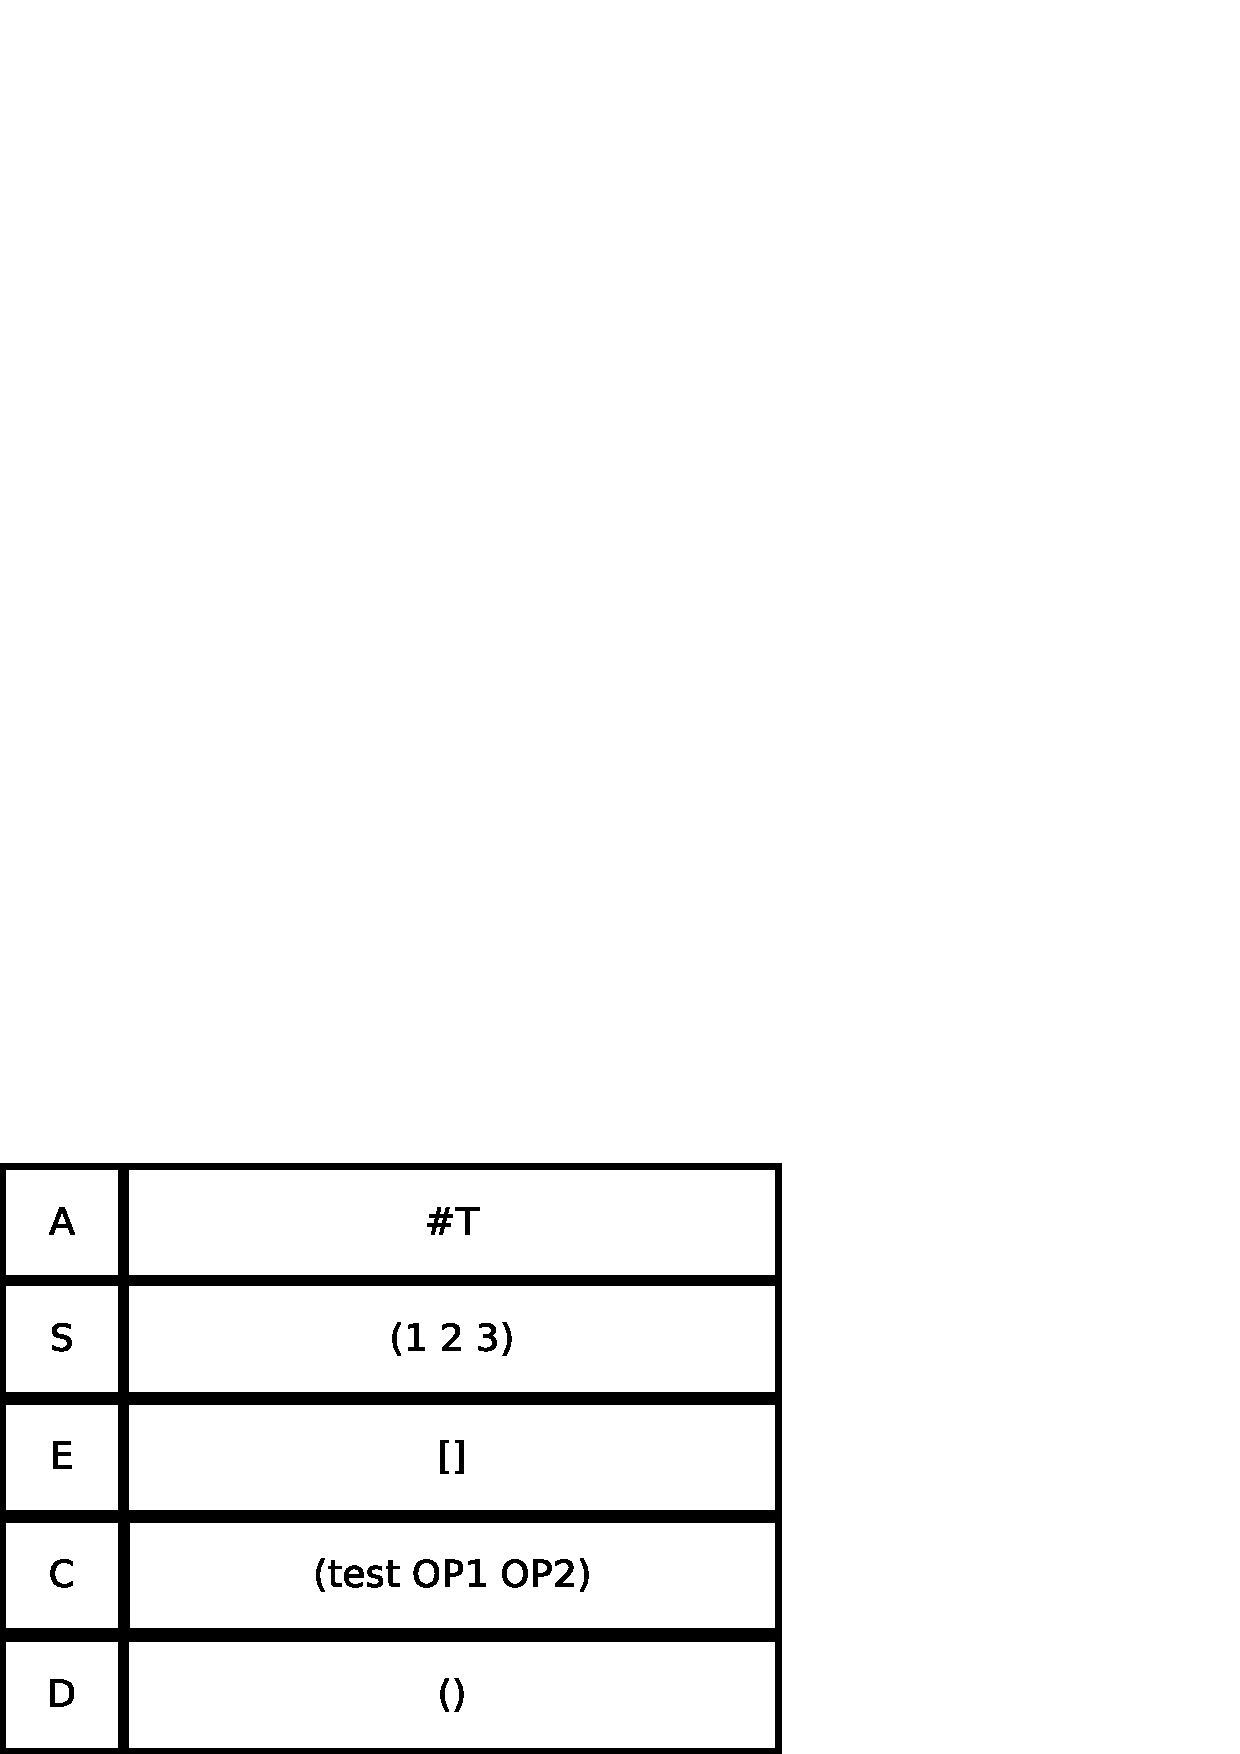
\includegraphics[width=.35\textwidth]{../images/maquina.pdf}
\caption{Estrutura da máquina quando da execução de uma instrução \sctt{test}}
\label{fig:maquina}
\end{figure}


\subsection{Instruções}
\label{ss:instrucoes}

A instrução \sctt{test} realiza controle de fluxo condicional, utilizando o
valor armazenado no \sctt{acumulador} e dois parâmetros chamados
\sctt{conseqüência} e \sctt{alternativa}. Ambos os parâmetros representam
trechos de código. Um exemplo de sua execução pode ser visto na figura
\ref{fig:op-test}

De acordo com o valor armazenado no \sctt{acumulador}, decide se deve continuar
a execução pela \sctt{consequência} (caso este valor seja diferente do literal
false) ou pela \sctt{alternativa} (caso este seja igual ao literal false),
armazenando no registrador \sctt{code} o valor escolhido entre os dois
parâmetros.

\begin{figure}[h!]
\centering
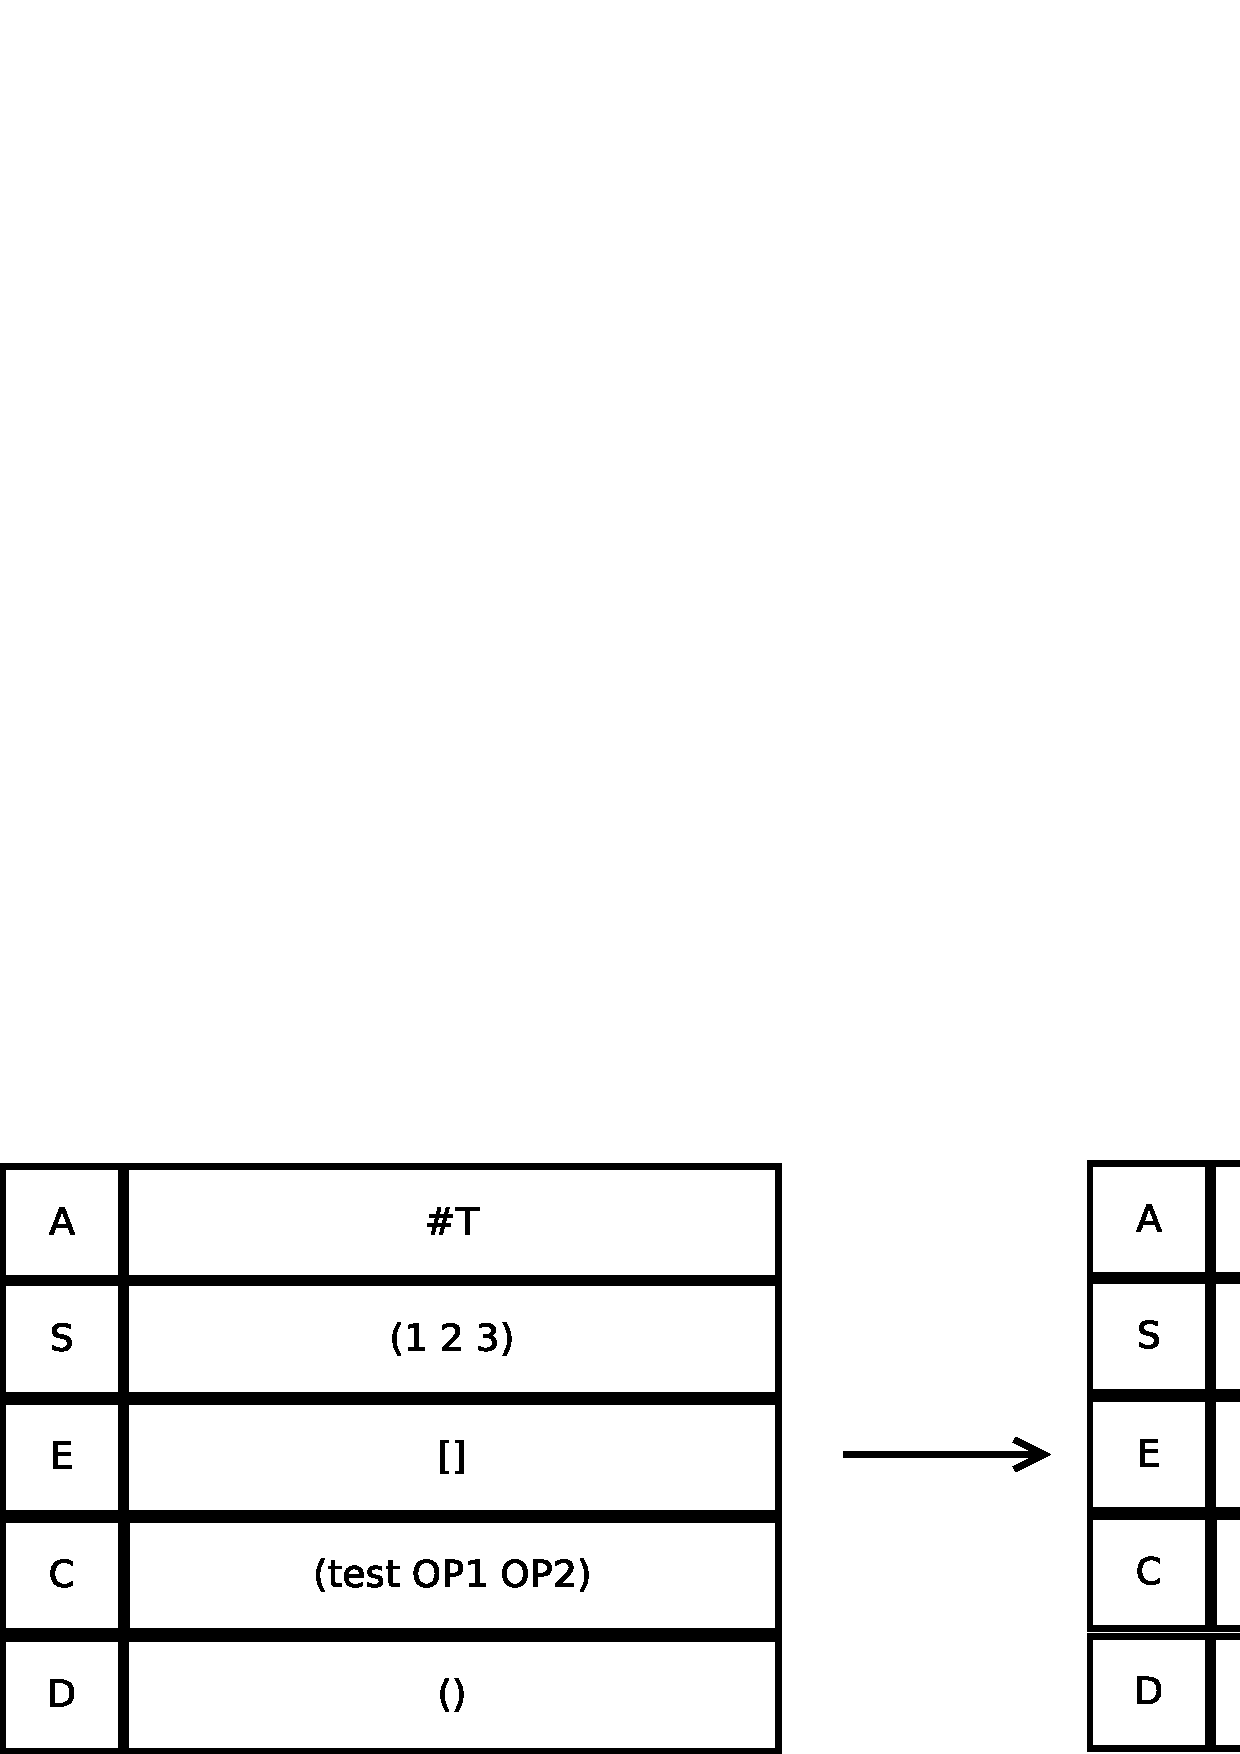
\includegraphics[width=.8\textwidth]{../images/op-test.pdf}
\caption{Comportamento da máquina ao executar uma instrução \sctt{test}}
\label{fig:op-test}
\end{figure}

A instrução \sctt{frame} é utilizada para salvar o estado da
máquina quando se faz necessária a execução de um outro procedimento,
armazenando o valor dos registradores atuais em uma pilha. Recebe dois
parâmetros: \sctt{retorno}, que indica o código que deve ser executado quando
este frame for restaurado, e \sctt{próximo}, que indica o código a ser
executado ao fim desta instrução.

Um novo frame é armazenado no registrador \sctt{dump}, contendo o valor dos
registradores \sctt{environment}, \sctt{stack} e \sctt{dump}, junto o valor do
parâmetro \sctt{retorno} que atua como valor do registrador \sctt{code} no
frame. Então o valor do registrador \sctt{stack} é setado para uma lista vazia
e o valor do registrador \sctt{code} é setado como o valor recebido no
parâmetro \sctt{próximo}. Um exemplo de sua execução pode ser visto na figura
\ref{fig:op-frame}.

A separação entre a instrução \sctt{frame} e a instrução \sctt{apply},
utilizada para invocar uma chamada de função, é crucial para a implementação da
eliminação de chamadas terminais: quando o compilador identifica que uma
chamada é terminal, simplesmente omite a criação de uma instrução \sctt{frame}.

\begin{figure}[h!]
\centering
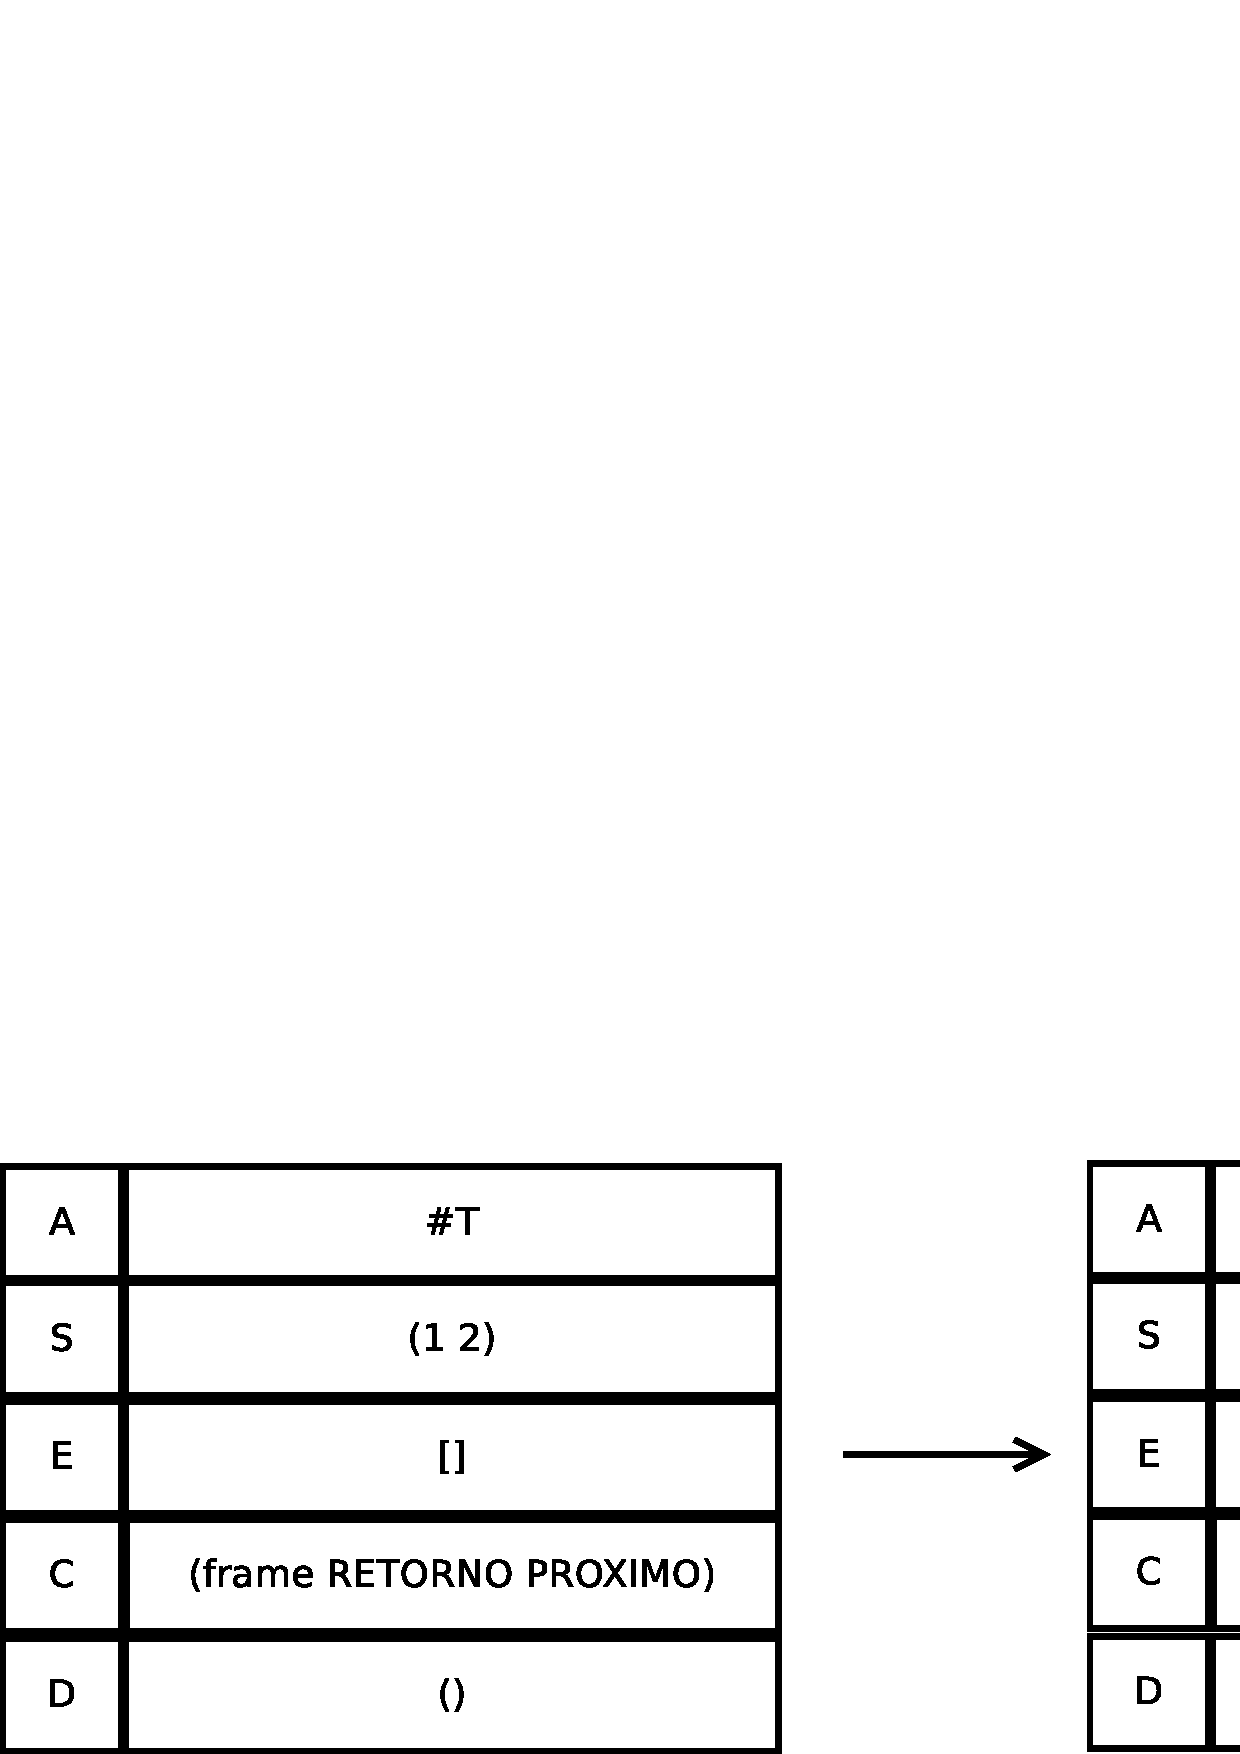
\includegraphics[width=.8\textwidth]{../images/op-frame.pdf}
\caption{Comportamento da máquina ao executar uma instrução \sctt{frame}}
\label{fig:op-frame}
\end{figure}


A instrução \sctt{constant}  carrega o valor de um literal
para utilização por outra instrução. Recebe dois parâmetros: \sctt{valor} e
\sctt{próximo}, que representam, respectivamente, o valor do literal a ser
carregado e o código a ser executado a seguir. O valor recebido como
\sctt{valor} substitui o valor no registrador \sctt{acumulador} e o valor em
\sctt{próximo} substitui o valor no registrador \sctt{code}. Um exemplo de sua execução pode ser visto na figura
\ref{fig:op-constant}.

\begin{figure}[h!]
\centering
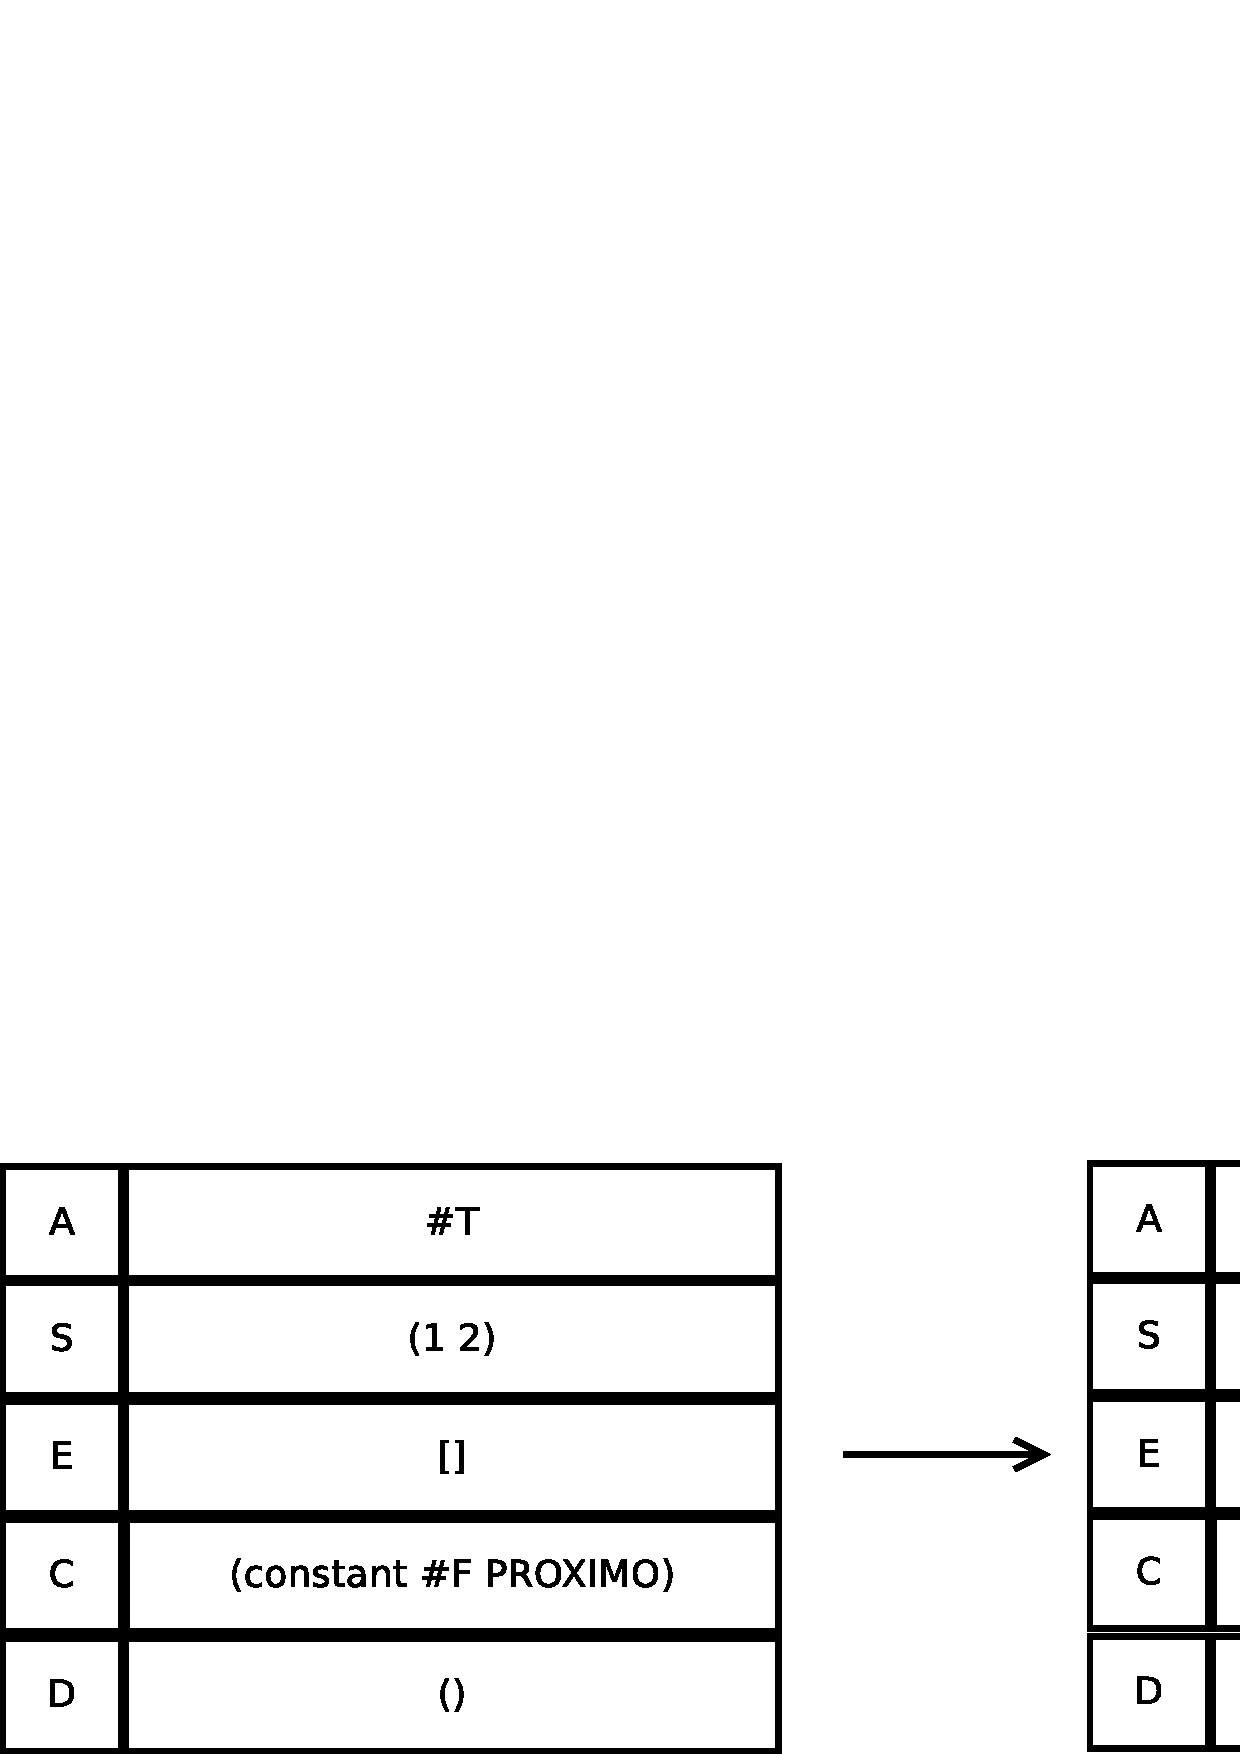
\includegraphics[width=.8\textwidth]{../images/op-constant.pdf}
\caption{Comportamento da máquina ao executar uma instrução \sctt{constant}}
\label{fig:op-constant}
\end{figure}


A instrução \sctt{lookup}  carrega o valor de uma variável
para o \sctt{acumulador}. Recebe dois parâmetros: \sctt{nome} e \sctt{próximo},
que representam o nome da variável a ser buscada e o código a ser executado a
seguir. O valor recebido como \sctt{nome} é utilizado para fazer a busca no
escopo de variáveis atual e o valor encontrado é então carregado no registrador
\sctt{acumulador}; o valor armazenado em \sctt{próximo} substitui o valor no
registrador \sctt{code}. Um exemplo de sua execução pode ser visto na figura
\ref{fig:op-lookup}.

\begin{figure}[h!]
\centering
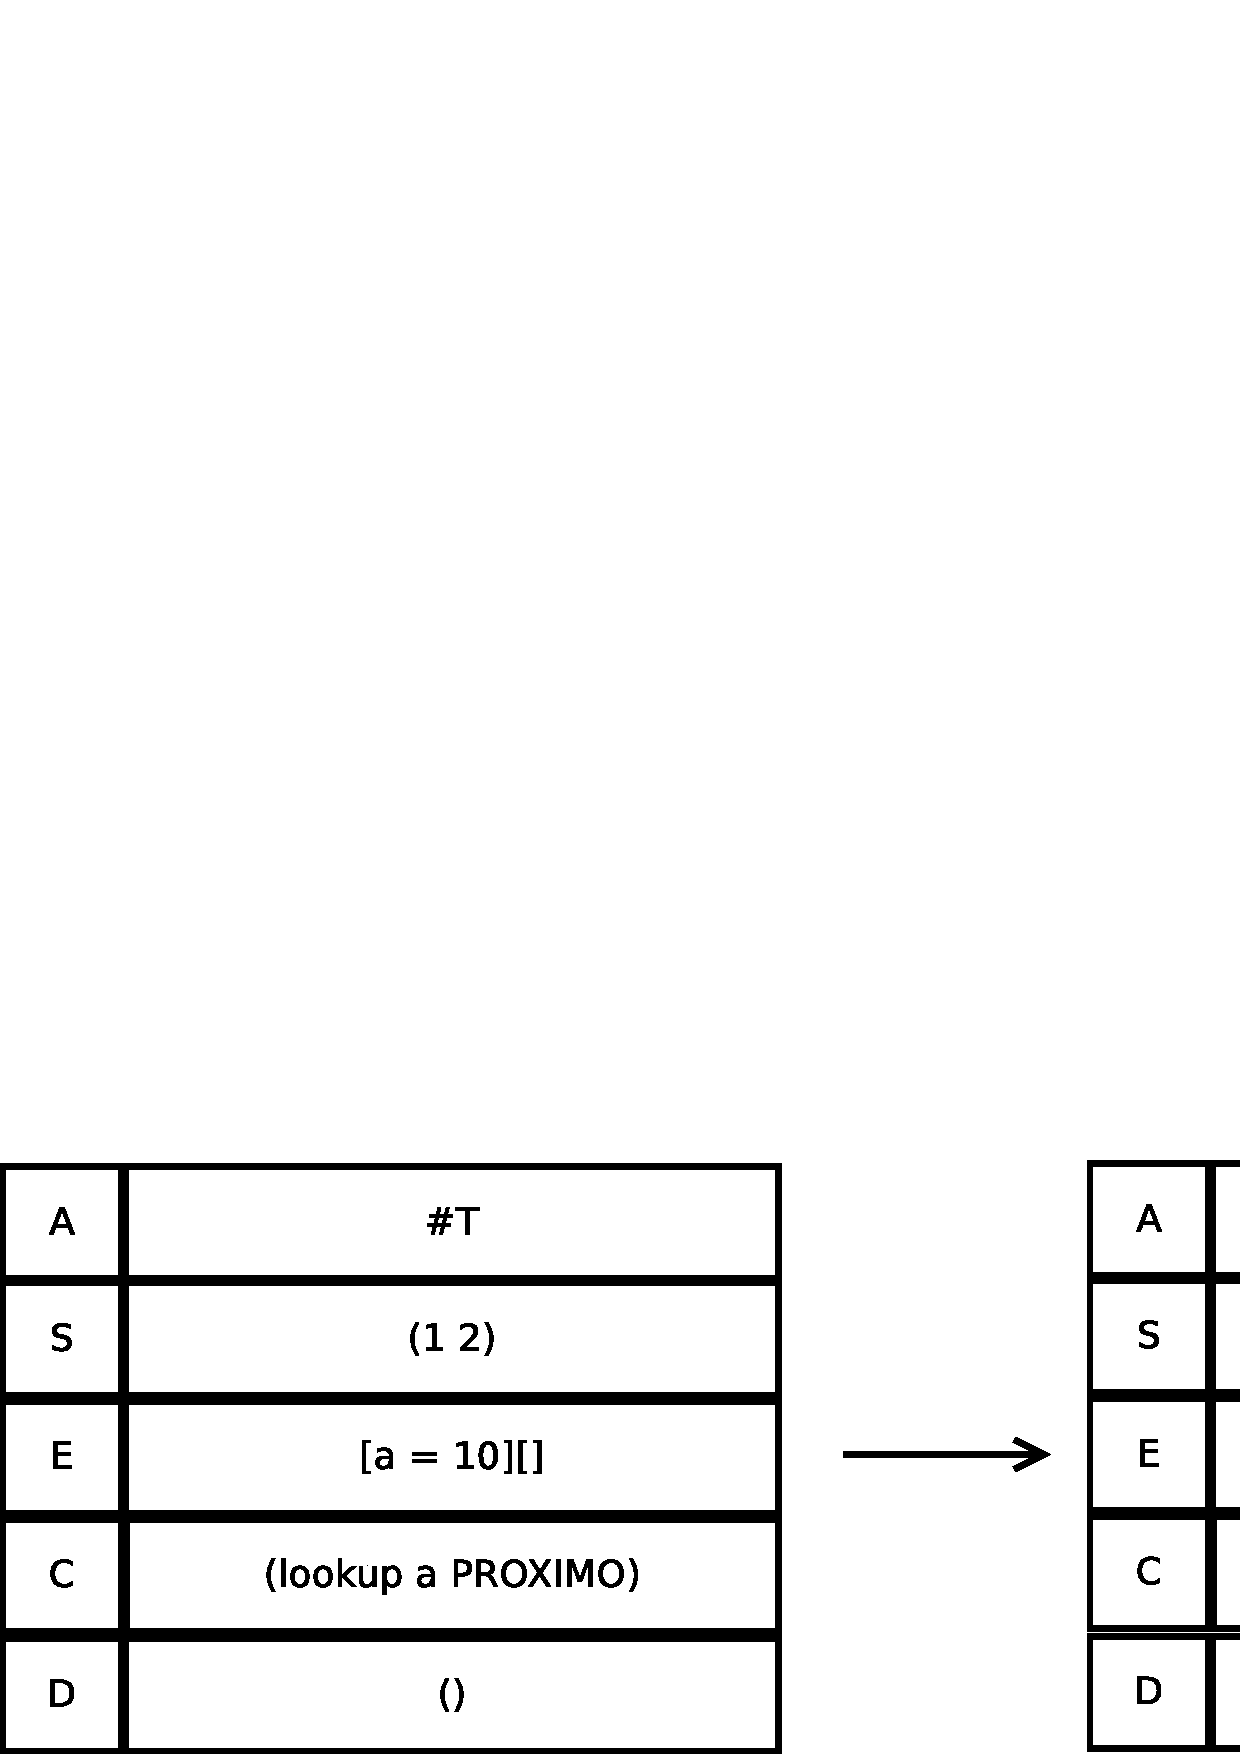
\includegraphics[width=.8\textwidth]{../images/op-lookup.pdf}
\caption{Comportamento da máquina ao executar uma instrução \sctt{lookup}}
\label{fig:op-lookup}
\end{figure}


A instrução \sctt{assign}  substitui o valor de uma variável
no escopo atual. Recebe dois parâmetros: \sctt{nome}, que representa o nome da
variável, e \sctt{próximo}, que indica o código a ser executado após a execução
da instrução atual. O valor da variável armazenada sob o vínculo indicado pelo
conteúdo de \sctt{nome} no escopo atual é substituído pelo valor no registrador
\sctt{acumulador}; caso não haja variável armazenada sob o nome indicado no
escopo atual, um erro é sinalizado.  O valor em \sctt{próximo} então substitui
o valor no registrador \sctt{code}. Um exemplo de sua execução pode ser visto na figura
\ref{fig:op-assign}.

\begin{figure}[h!]
\centering
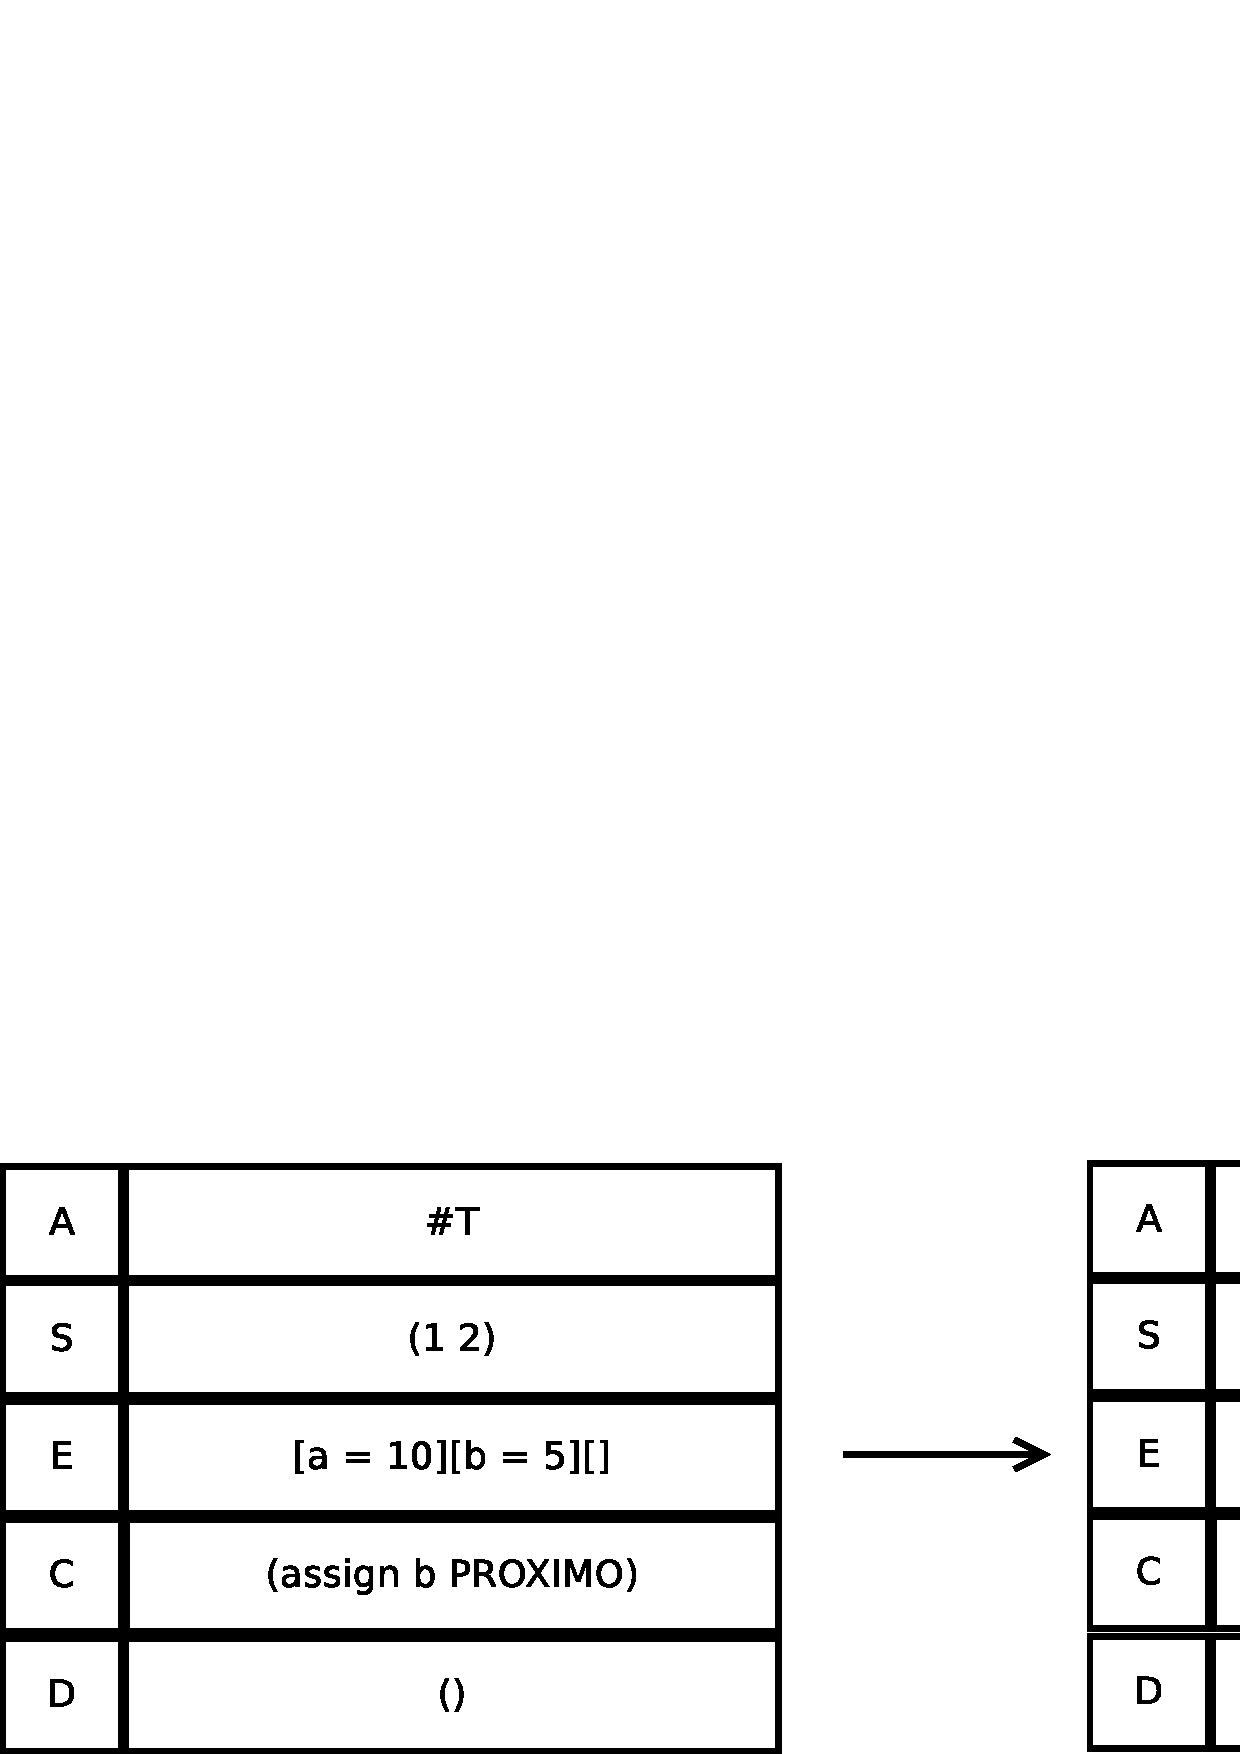
\includegraphics[width=.8\textwidth]{../images/op-assign.pdf}
\caption{Comportamento da máquina ao executar uma instrução \sctt{assign}}
\label{fig:op-assign}
\end{figure}


A instrução \sctt{bind}  cria, no nível mais próximo do escopo
atual, um novo vínculo de variável. Funciona de modo quase idêntico à instrução
\sctt{assign} recebendo os mesmos parâmetros, com a diferença que caso não haja
variável armazenada sob o nome indicado, uma variável é criada para conter o
valor. Um exemplo de sua execução pode ser visto na figura
\ref{fig:op-bind}.

\begin{figure}[h!]
\centering
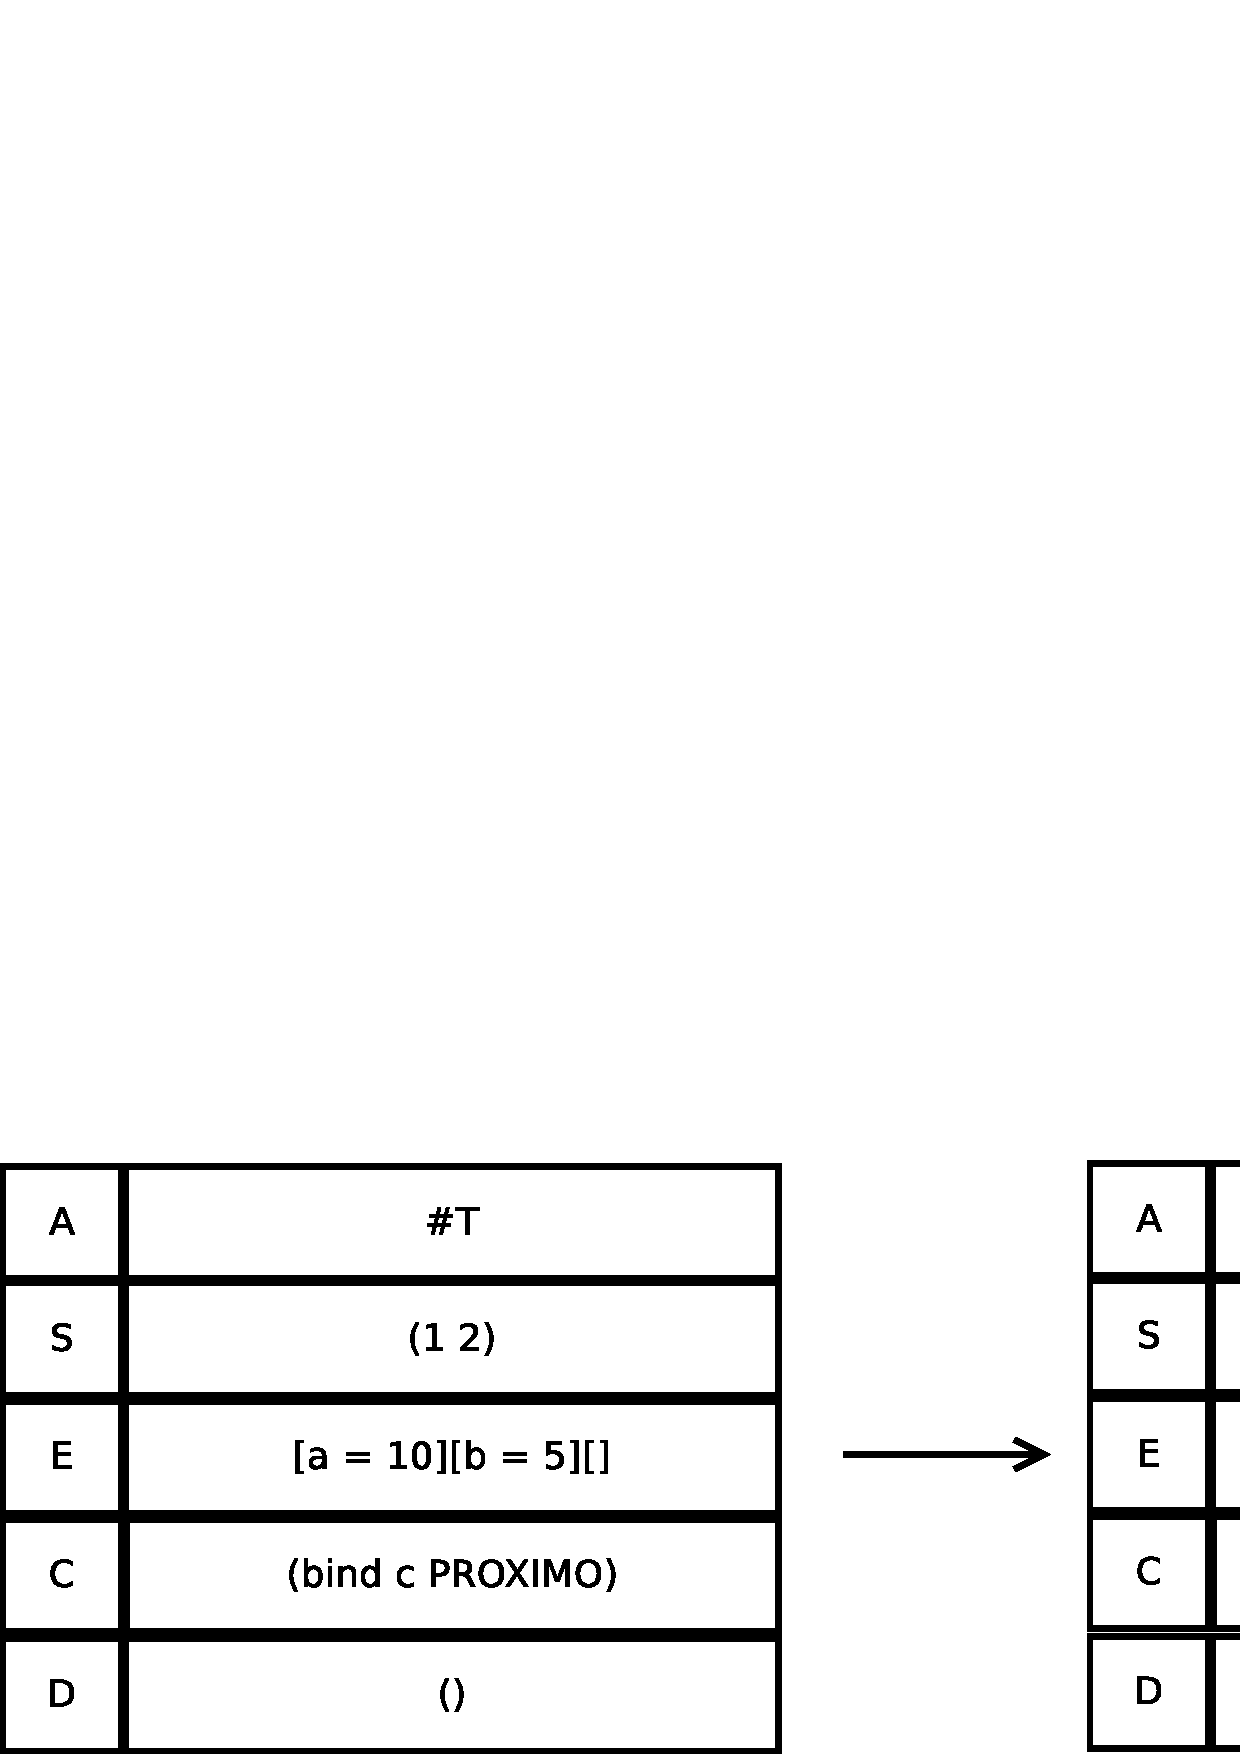
\includegraphics[width=.8\textwidth]{../images/op-bind.pdf}
\caption{Comportamento da máquina ao executar uma instrução \sctt{bind}}
\label{fig:op-bind}
\end{figure}


A instrução \sctt{argument}  armazena na pilha do
registrador \sctt{stack} o valor atual do \sctt{acumulador}. Recebe apenas o
parâmetro \sctt{próximo} indicando qual o código a ser executado a seguir, que
então é utilizado para configurar o registrador \sctt{code}.  Um exemplo de sua execução pode ser visto na figura
\ref{fig:op-argument}.


\begin{figure}[h!]
\centering
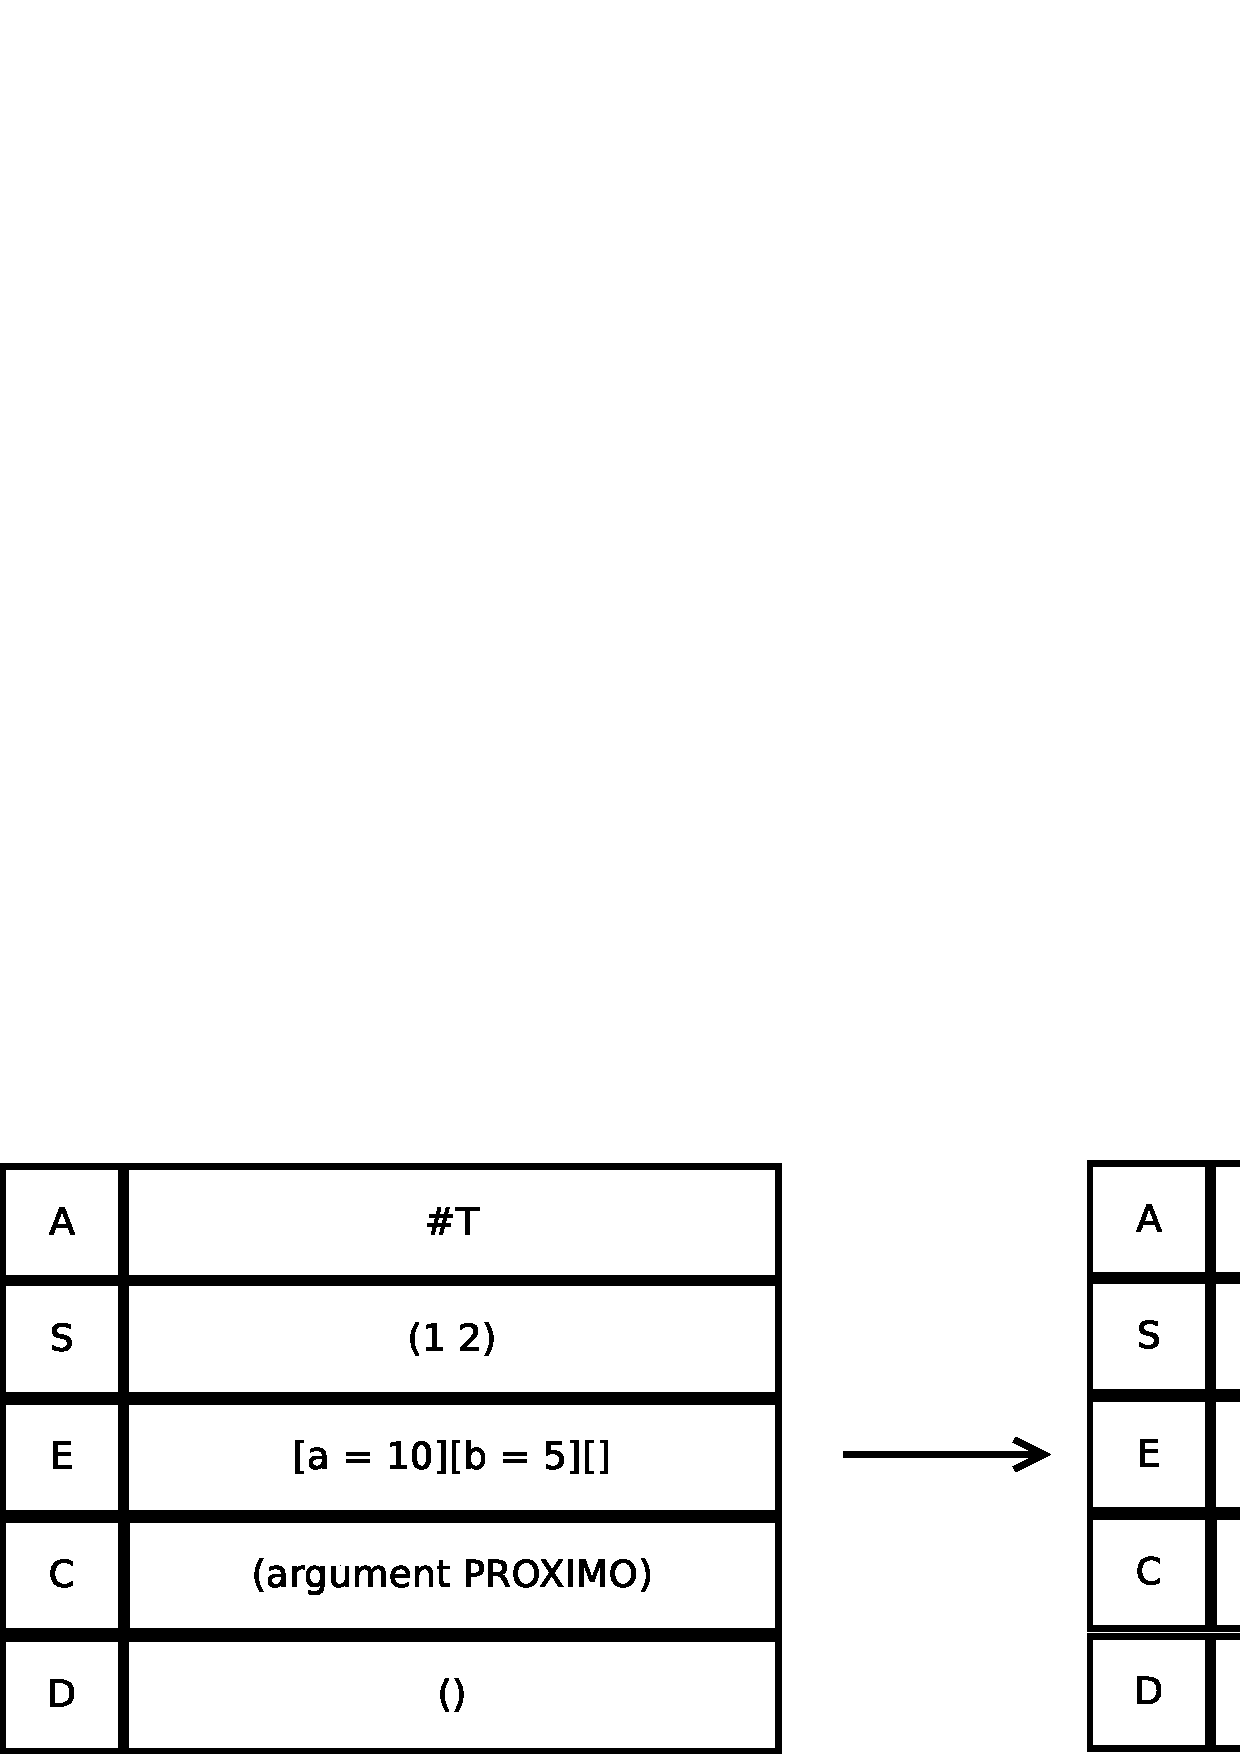
\includegraphics[width=.8\textwidth]{../images/op-argument.pdf}
\caption{Comportamento da máquina ao executar uma instrução \sctt{argument}}
\label{fig:op-argument}
\end{figure}


A instrução \sctt{apply}  inicia uma chamada a uma função ou primitiva e não
recebe parâmetro algum. Utiliza como indicador de qual função ou primitiva a
ser chamado o valor atual do \sctt{acumulador}. Um exemplo de sua execução pode
ser visto na figura \ref{fig:op-apply}. 

Caso o valor no \sctt{acumulador} represente uma primitiva, a instrução
simplesmente passa ao código da primtiiva a lista de parâmetros e mais nada. No
entanto, se o valor no \sctt{acumulador} representar uma função ou closure
definida pelo usuário um novo contexto de escopo baseado no valor dos
argumentos e os parâmetros da função é criado e substitui o valor em
\sctt{environment}, o registrador \sctt{stack} recebe uma lista vazia e o valor
do registrador \sctt{code} é substituido pelo código da função em questão. 

\begin{figure}[h!]
\centering
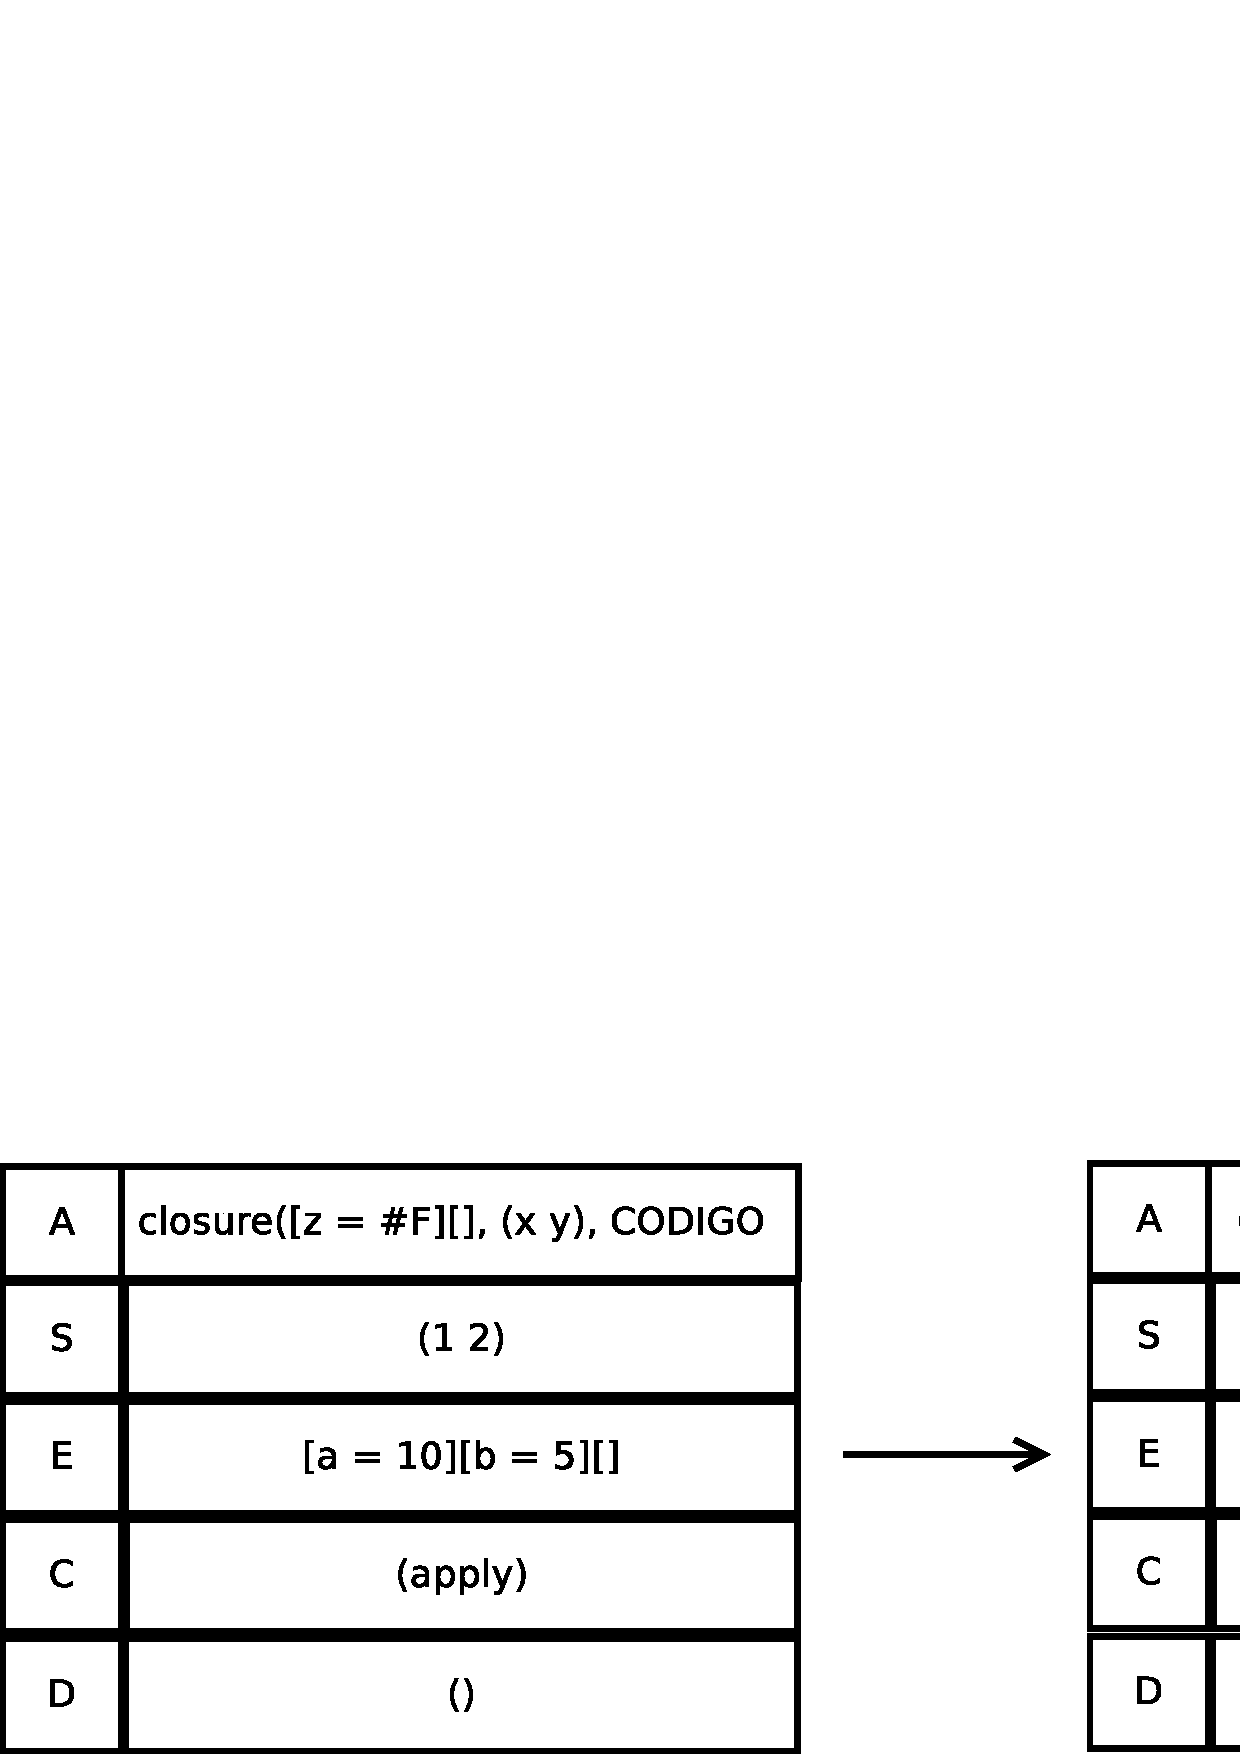
\includegraphics[width=.8\textwidth]{../images/op-apply.pdf}
\caption{Comportamento da máquina ao executar uma instrução \sctt{apply}}
\label{fig:op-apply}
\end{figure}


A instrução \sctt{return}  restaura um frame anteriormente salvo pela instrução
\sctt{frame}. Não recebe parâmetro algum e configura os valores dos
registradores \sctt{stack}, \sctt{environment}, \sctt{code} e \sctt{dump} para
os valores contidos no primeiro elemento da pilha armazenada no registrador
\sctt{dump}. Mantém o registrador \sctt{acumulador} intacto. Um exemplo de sua
execução pode ser visto na figura \ref{fig:op-return}. 

\begin{figure}[h!]
\centering
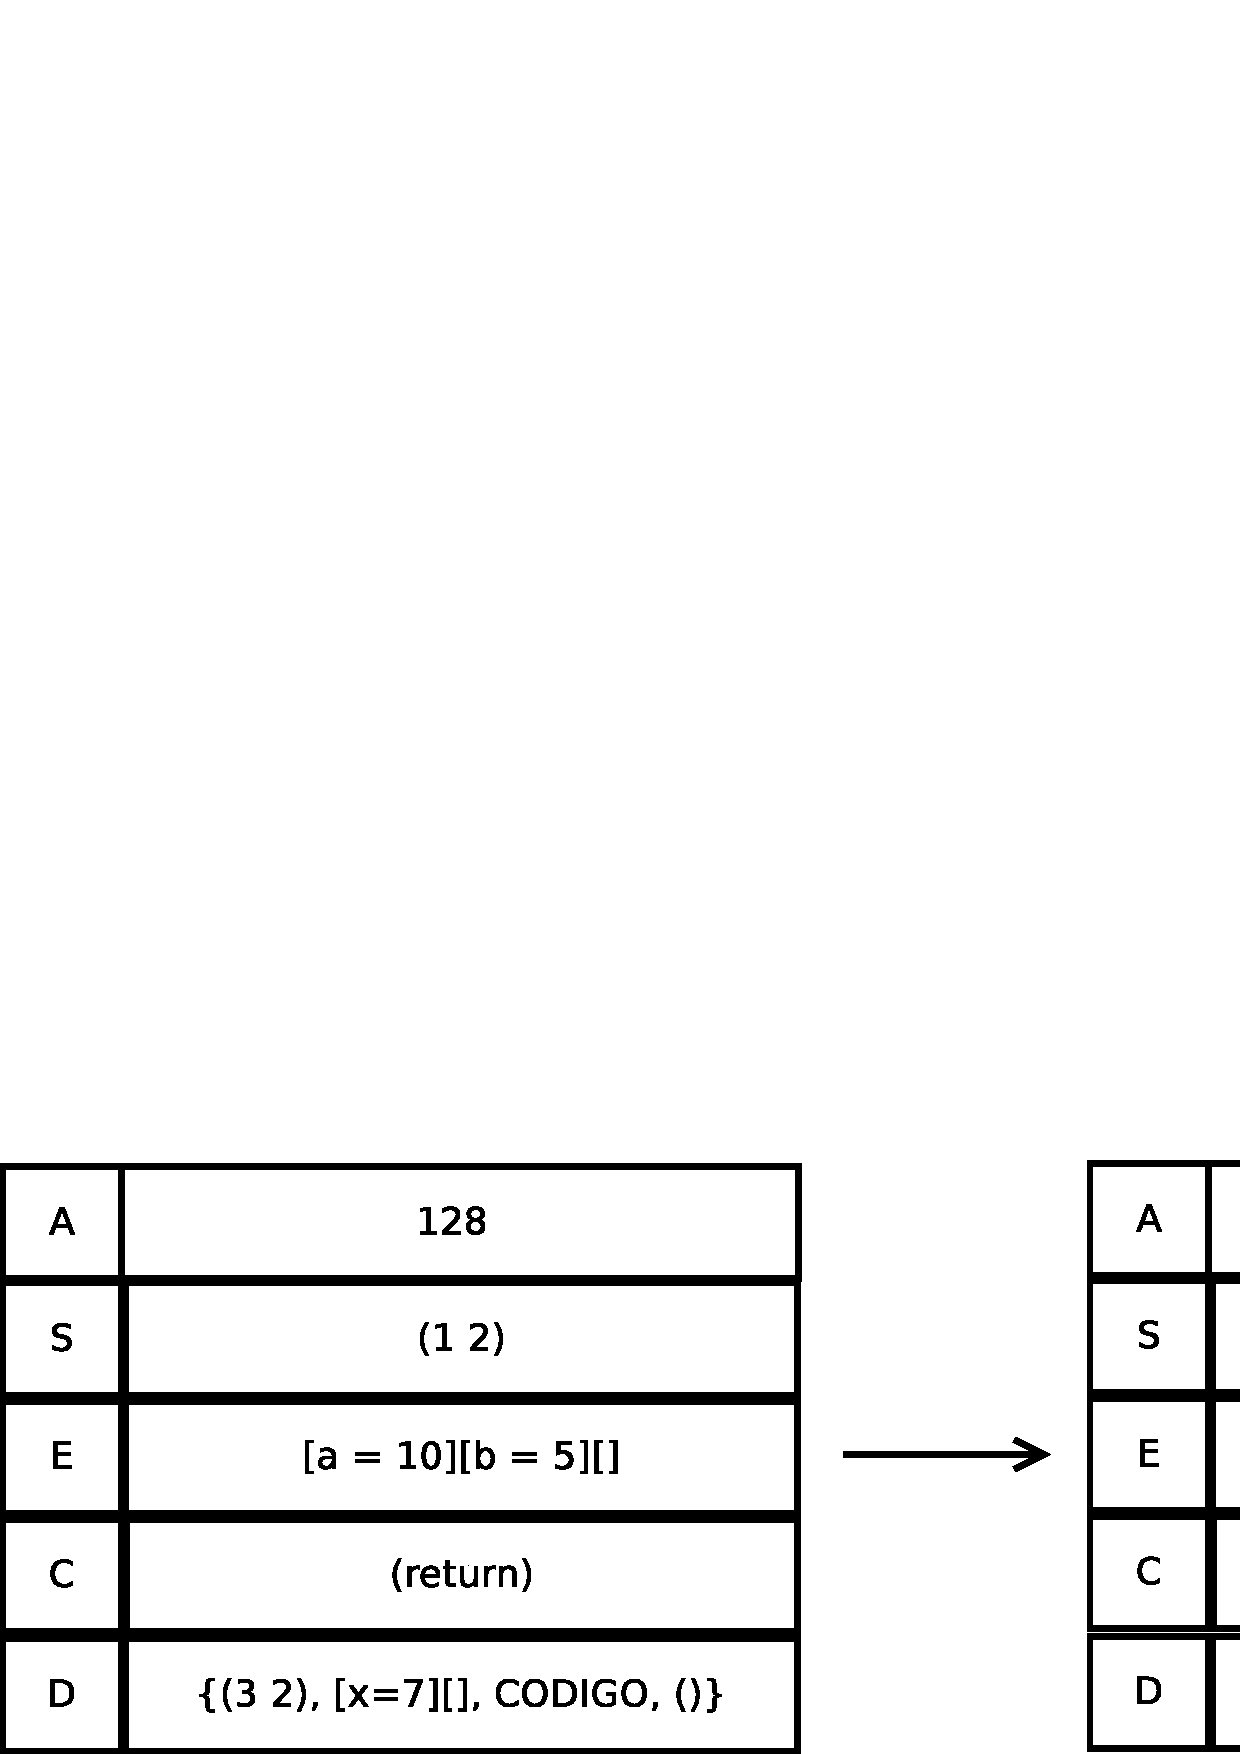
\includegraphics[width=.8\textwidth]{../images/op-return.pdf}
\caption{Comportamento da máquina ao executar uma instrução \sctt{return}}
\label{fig:op-return}
\end{figure}


A instrução \sctt{reify}  é utilizada para restaurar a
computação ao ponto de uma continuação previamente obtida. Recebe como
parâmetros \sctt{dump} e \sctt{valor}, que representam, respectivamente, o
conteúdo do registrador \sctt{dump} no momento da criação da continuação e o
valor a ser restaurado para o \sctt{acumulador} quando a continuação for
restaurada. O efeito final da instrução, é o de retornar ao ponto em que a
continuação foi criada, restaurando os valores presentes no primeiro elemento
da pilha em \sctt{dump}, deixando \sctt{valor} no \sctt{acumulador}. Um exemplo de sua
execução pode ser visto na figura \ref{fig:op-reify}. 

\begin{figure}[h!]
\centering
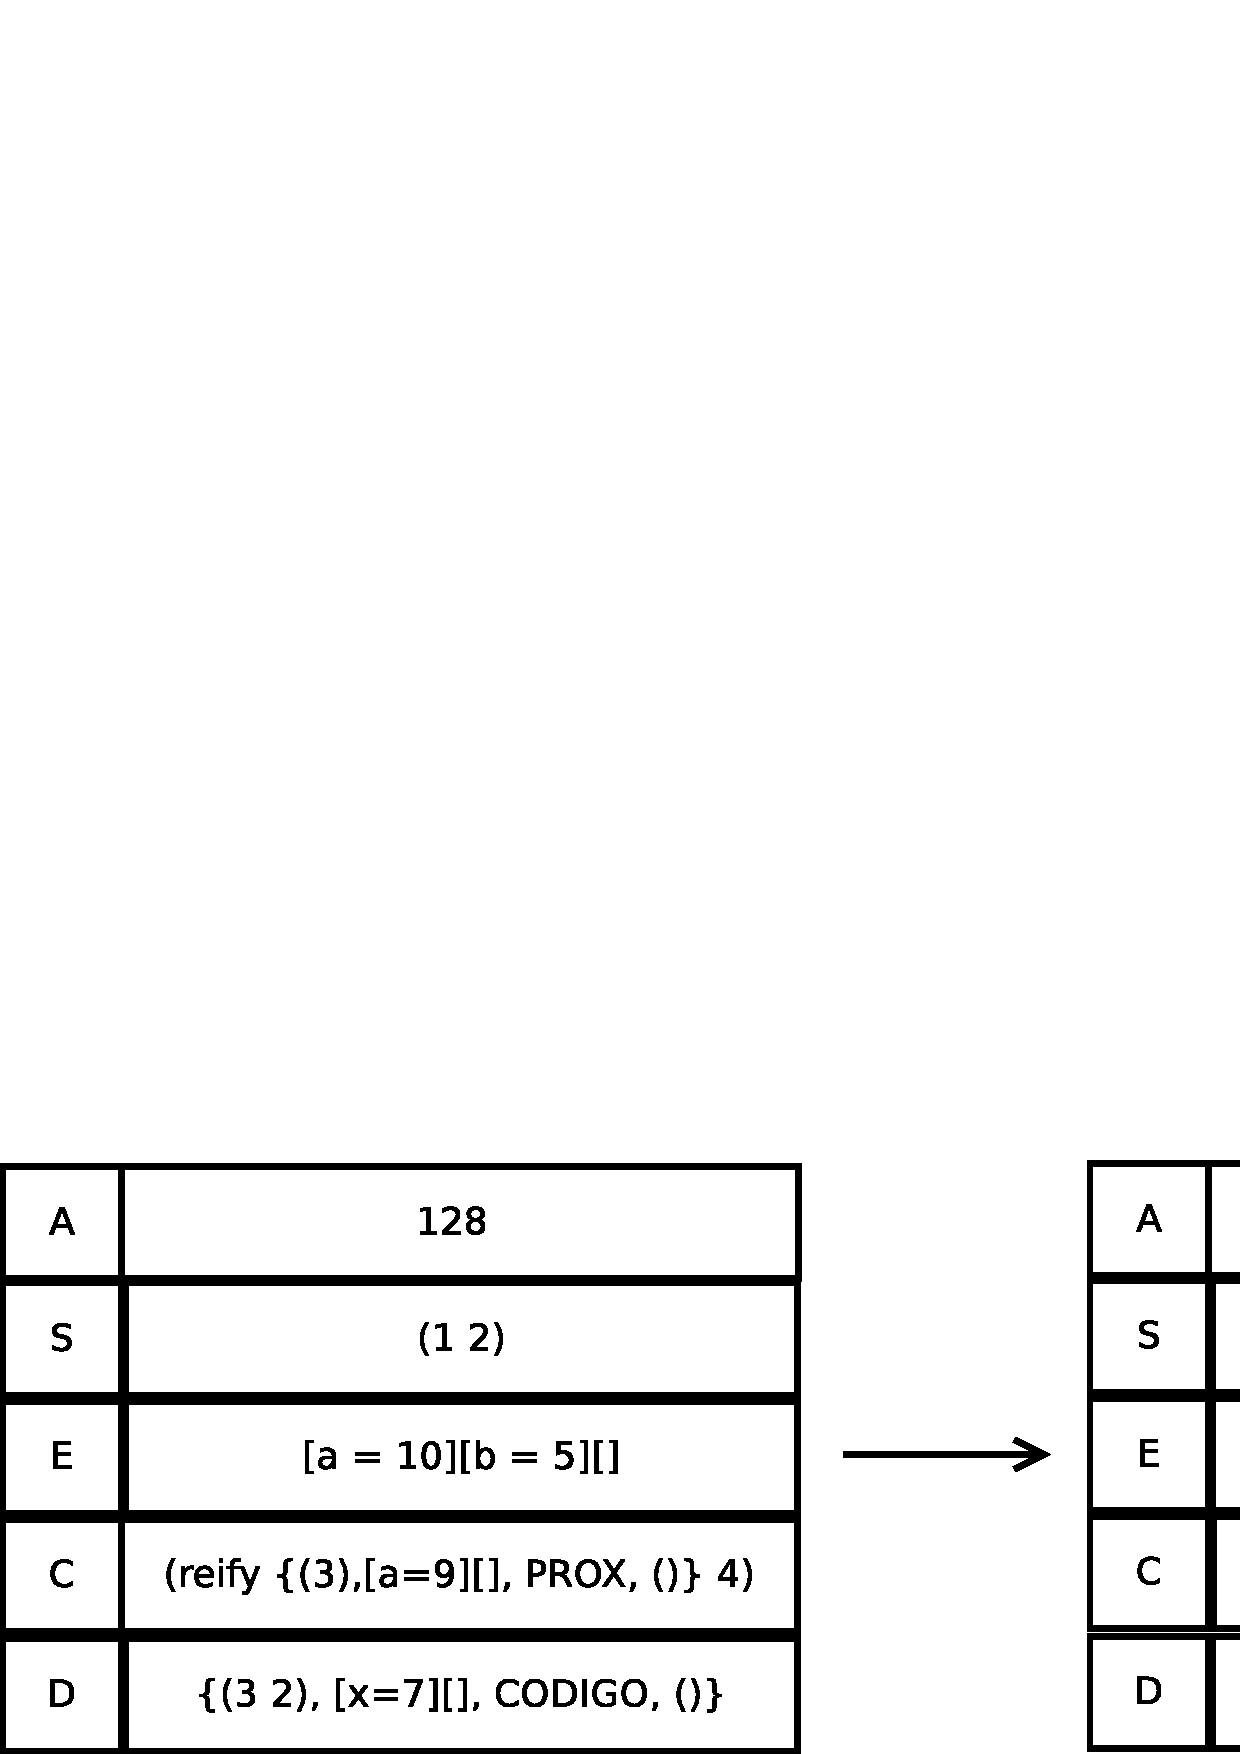
\includegraphics[width=.8\textwidth]{../images/op-reify.pdf}
\caption{Comportamento da máquina ao executar uma instrução \sctt{reify}}
\label{fig:op-reify}
\end{figure}


A instrução \sctt{save}  é responsável por criar uma referência
para a continuação da computação atual. Recebe apenas um parâmetro,
\sctt{próximo}, que é indica qual a próxima instrução a ser executada ao fim
desta. Com a arquitetura utilizada pela máquina virtual, uma continuação é
simplesmente uma closure de apenas um parâmetro, contendo o valor atual do
registrador \sctt{dump} encapsulado, cujo único efeito é chamar a instrução
\sctt{reify} com parâmetros o valor do registrador \sctt{dump} quando a
continuação foi criada e o valor do único parâmetro da closure. Esta closure é
então armazenada no \sctt{acumulador}.

A instrução \sctt{closure}  cria uma nova closure, uma função
em que o contexto na qual foi criada é acessível. Recebe como parâmetros
\sctt{argumentos}, \sctt{corpo} e \sctt{proximo} que são, respectivamente, uma
lista contendo os parâmetros formais da closure a ser criada, o código
compilado do corpo da função e o endereço do código que deve ser executado ao
fim desta instrução. A nova closure criada é armazenada no \sctt{acumulador} e
o registrador \sctt{code} é configurado com o valor de \sctt{próximo}. Um exemplo de sua
execução pode ser visto na figura \ref{fig:op-closure}. 

\begin{figure}[h!]
\centering
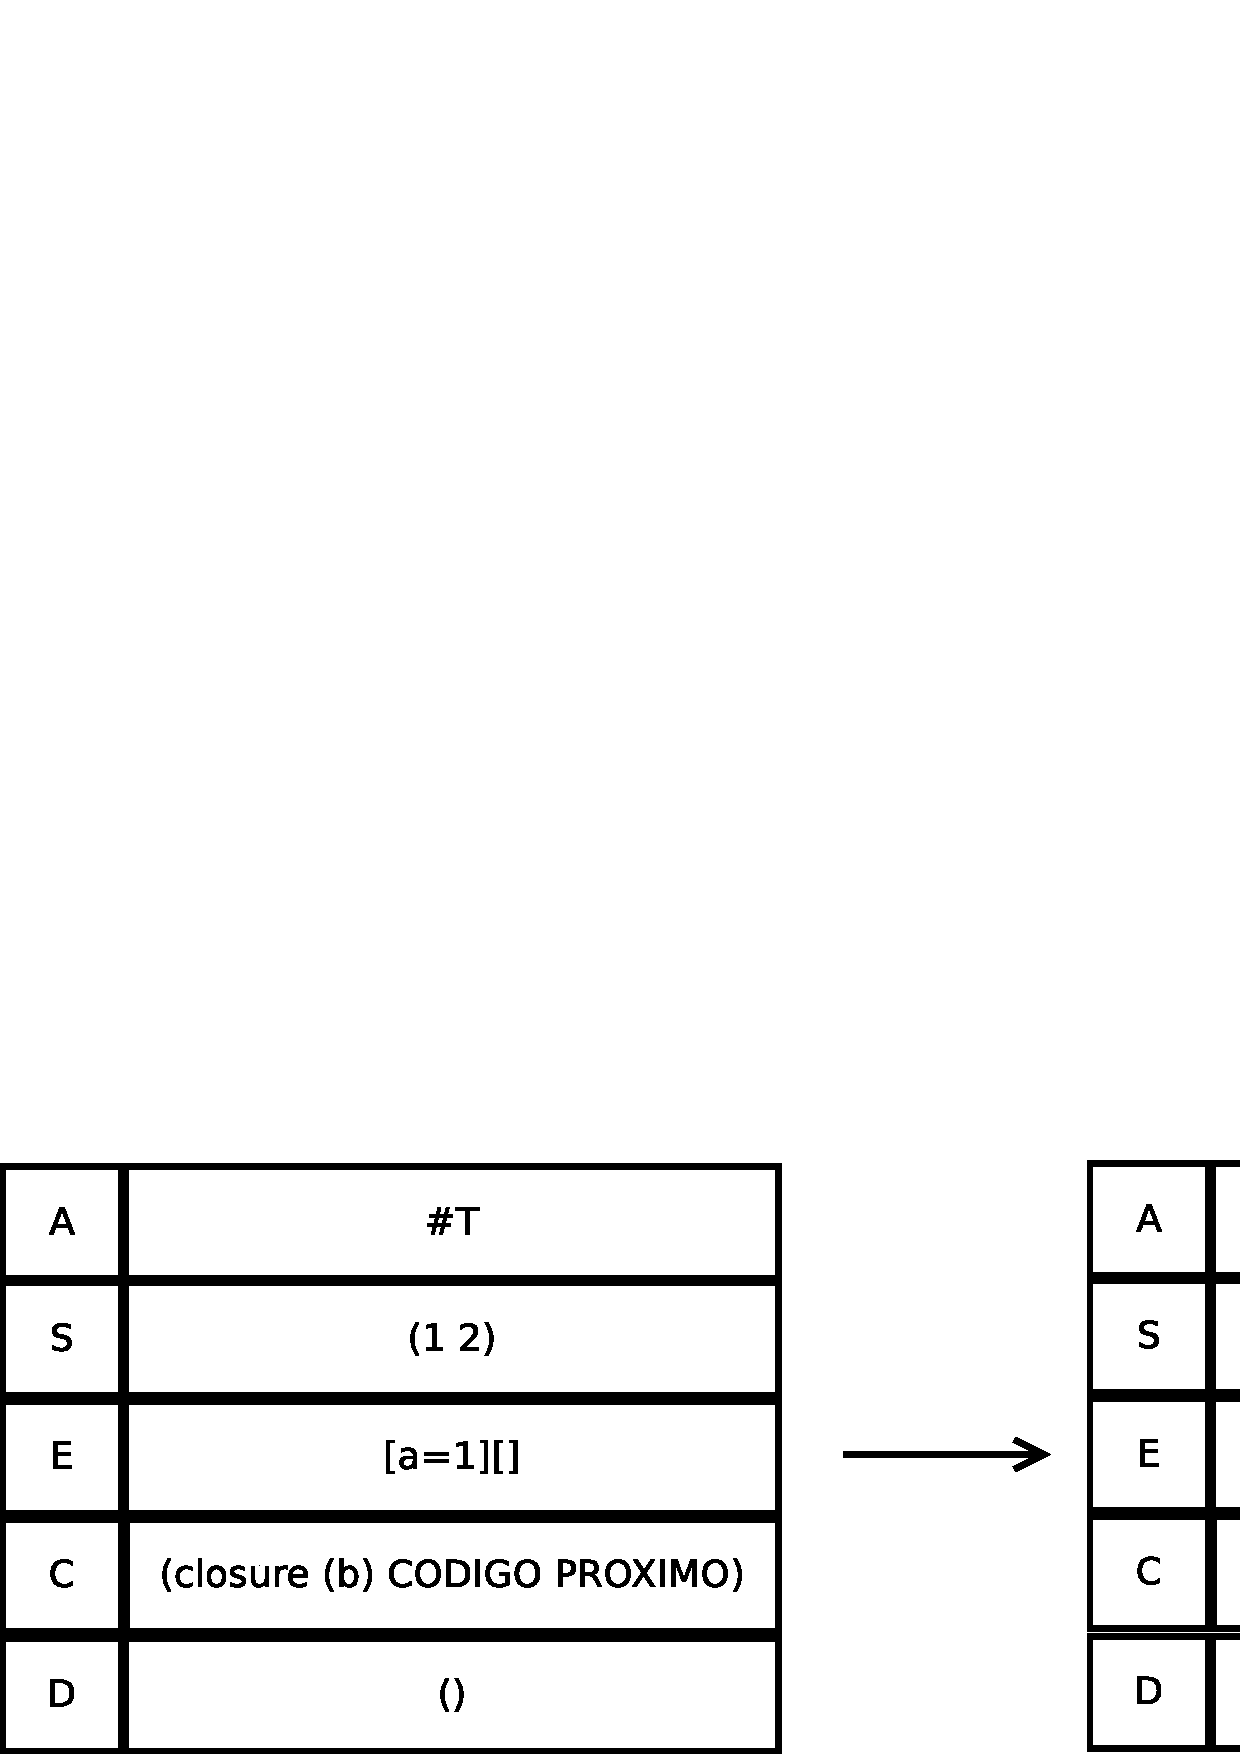
\includegraphics[width=.8\textwidth]{../images/op-closure.pdf}
\caption{Comportamento da máquina ao executar uma instrução \sctt{closure}}
\label{fig:op-closure}
\end{figure}


A instrução \sctt{bind-macro} é uma variante próxima da instrução \sctt{bind},
usada apenas para mitigar uma deficiência do compilador: a falta de um
mecanismo em tempo de compilação para gerenciar macros. Esta instrução recebe
dois parâmetros, \sctt{nome} e \sctt{proximo}, e espera que o \sctt{acumulador}
contenha código para uma macro. Como resultado, guarda em um contexto geral de
macros uma referência para o código da macro sob o nome recebido como
\sctt{nome} e substitui o valor em \sctt{code} pelo valor de \sctt{proximo}.

A última instrução, \sctt{halt}, simplesmente indica à máquina virtual que o
processamento está terminado, e que o valor no \sctt{acumulador} deve ser
retornado como resultado da computação. Não recebe parâmetro algum, e não
altera registrador algum.





\end{document}

% vim:filetype=tex ts=4 sw=4 noet tw=76
